\documentclass[twoside]{article}
\usepackage{icml2017}

% If your paper is accepted, change the options for the package
% aistats2015 as follows:
%
%\usepackage[accepted]{aistats2015}
%
% This option will print headings for the title of your paper and
% headings for the authors names, plus a copyright note at the end of
% the first column of the first page.

%%%%%%%%%%%%%%%%%%%%%%%%%%%%%%%%%%%%%%%%%%%%%%%%%%%%%%%%%%%%%%%%%%%%%%%%%%%%%%%%

\usepackage{amsmath}
\usepackage{amssymb}
\usepackage{amsthm}
\usepackage{mathtools}
\usepackage{graphicx}
\usepackage{rotating}
\usepackage{xcolor}
\usepackage[inline]{enumitem}

%\usepackage{algorithm}
%\usepackage[noend]{algpseudocode}
%\usepackage{algorithmicx}
%\usepackage{algorithm2e}

%\usepackage[authordate,bibencoding=auto,strict,backend=biber,natbib]{biblatex-chicago}
%\usepackage[round]{natbib}   % omit 'round' option if you prefer square brackets
%\bibliographystyle{plainnat}

\usepackage{tikz}
\usepackage{pgfplots}
\pgfplotsset{width=7cm,compat=1.8}
\definecolor{darkgreen}{RGB}{0,127,0}

%%%%%%%%%%%%%%%%%%%%%%%%%%%%%%%%%%%%%%%%

\newtheorem{cor}{Corollary}
\newtheorem{theorem}{Theorem}
\newtheorem{lemma}{Lemma}
\newtheorem{assumption}{Condition}
\newtheorem{defn}{Definition}

\DeclareMathOperator*{\argmin}{arg\,min}
\DeclareMathOperator*{\argmax}{arg\,max}
\DeclareMathOperator*{\vecspan}{span}
\DeclareMathOperator*{\affspan}{aff}
\DeclareMathOperator*{\subG}{subG}
\DeclareMathOperator*{\tr}{tr}

%\newcommand{\smin}[1]{s_\text{min}({#1})}
\newcommand{\smin}{s_\text{min}}
\newcommand{\smax}{s_\text{max}}
\newcommand{\qhi}{q_\text{hi}}
\newcommand{\qlo}{q_\text{lo}}
\newcommand{\zero}{\text{\textbf{0}}}
\newcommand{\Zproj}{Z^{\textit{proj}}}
\newcommand{\Zowa}{Z^{\textit{owa}}}
\newcommand{\nowa}{n^{\textit{owa}}}
\newcommand{\Q}{\mathcal{Q}}
\newcommand{\Y}{\mathcal{Y}}
\newcommand{\X}{\mathcal{X}}
\newcommand{\matW}{\hat W}
\newcommand{\matV}{\hat V}
\newcommand{\W}{{\mathcal W}}
\newcommand{\Wowa}{{\hat \W^{\textit{owa}}}}
\newcommand{\Waff}{\mathcal{\hat A}}
\newcommand{\WaffE}{{\mathcal{\hat A}_\E}}
\newcommand{\Wave}{{\mathcal{\hat W}^{ave}}}
\newcommand{\Wtave}{{\mathcal{W}^{ave,*}}}
\newcommand{\V}{\mathcal{V}}
\newcommand{\A}{\mathcal{A}}
\newcommand{\D}{\mathcal{D}}
\newcommand{\E}{\mathbb{E}}
\newcommand{\x}{\mathbf{x}}
\newcommand{\y}{\mathbf{y}}
\newcommand{\w}{\mathbf w}
\newcommand{\vv}{\mathbf{v}}
\newcommand{\vfull}{\hat\vv^{\textit{owa,full}}}
\newcommand{\vowa}{\hat\vv^{\textit{owa}}}
\newcommand{\wkl}{\hat\w^{kl}}
\newcommand{\astar}{\vv^*}
\newcommand{\wowa}{\hat\w^{owa}}
\newcommand{\wowafull}{\hat\w^{\textit{owa,full}}}
\newcommand{\wowastar}{\hat\w^{\textit{owa,*}}}
\newcommand{\wave}{\hat\w^{ave}}
\newcommand{\wtave}{\E\hat\w^{ave}}
\newcommand{\waver}{\hat\w^{ave,r}}
\newcommand{\wboot}{\hat\w^{boot}}
\newcommand{\wmle}{\hat\w^{erm}}
\newcommand{\wmler}{\hat\w^{erm,r}}
\newcommand{\wstar}{{\w^{*}}}
\newcommand{\what}{{\hat\w}}
\newcommand{\wq}{\hat\w^{q}}
\newcommand{\wqstar}{\hat\w^{q^*}}
\newcommand{\dist}{\mathcal{D}}
\newcommand{\reg}{r}
\newcommand{\loss}{\ell}
\newcommand{\Loss}{\mathcal{L}}

\newcommand{\tbias}{t_{\text{\textit{bias}}}}
\newcommand{\tvar}{t_{\text{\textit{var}}}}

\newcommand{\I}{\mathcal I}
%\newcommand{\I^{-1}}{\I^{-1}}
\newcommand{\law}{\ensuremath{\xrightarrow{L}}}
\newcommand{\normal}[2]{\ensuremath{\mathcal{N}\left({{#1}},{{#2}}\right)}}
\newcommand{\subnormal}[1]{\ensuremath{\subG\left({{#1}}\right)}}
\newcommand{\trans}[1]{\ensuremath{{#1}^{\mathsf{T}}}}
\newcommand{\pinv}[1]{\ensuremath{{#1}^{\mathsf{\dagger}}}}
\newcommand{\ltwo}[1]{{\lVert {#1} \rVert}}
\newcommand{\ltwobig}[1]{{\left\lVert {#1} \right\rVert}}
\newcommand{\lone}[1]{{\lVert {#1} \rVert}_1}
\newcommand{\lzero}[1]{{\lVert {#1} \rVert}_0}
\newcommand{\proj}[1]{\pi_{{#1}}}
\newcommand{\prob}[1]{\Pr\left[{#1}\right]}

\DeclarePairedDelimiterX{\infdivx}[2]{(}{)}{%
  #1\;\delimsize\|\;#2%
}
\newcommand{\kl}{\text{KL}\infdivx}

%\newcommand{\plots}[1]{}
\newcommand{\plots}[1]{#1}
\newcommand{\ignore}[1]{}
\newcommand{\fixme}[1]{\textbf{FIXME:} {#1}}

%%%%%%%%%%%%%%%%%%%%%%%%%%%%%%%%%%%%%%%%%%%%%%%%%%%%%%%%%%%%%%%%%%%%%%%%%%%%%%%%

\begin{filecontents}{paper.bib}

@article{scikit-learn,
 title={Scikit-learn: Machine Learning in {P}ython},
 author={Pedregosa, F. and Varoquaux, G. and Gramfort, A. and Michel, V.
         and Thirion, B. and Grisel, O. and Blondel, M. and Prettenhofer, P.
         and Weiss, R. and Dubourg, V. and Vanderplas, J. and Passos, A. and
         Cournapeau, D. and Brucher, M. and Perrot, M. and Duchesnay, E.},
 journal={Journal of Machine Learning Research},
 volume={12},
 pages={2825--2830},
 year={2011}
}

@article{kddcup2012,
  author={Yanzhi Niu and Yi Wang and Gordon Sun and Aden Yue and Brian Dalessandro and Claudia Perlich and Ben Hamner},
  title = {The Tencent Dataset and {KDD}-Cup'12},
  howpublished = {URL \url{http://www.kddcup2012.org/c/kddcup2012-track2}},
  year = {2012}
}

@book{lehmann1999elements,
  title={Elements of large-sample theory},
  author={Lehmann, Erich Leo},
  year={1999},
  publisher={Springer Science \& Business Media}
}

@inproceedings{merugu2003privacy,
  title={Privacy-preserving distributed clustering using generative models},
  author={Merugu, Srujana and Ghosh, Joydeep},
  booktitle={Data Mining, 2003. ICDM 2003. Third IEEE International Conference on},
  pages={211--218},
  year={2003},
  organization={IEEE}
}

@article{dasgupta2003elementary,
  title={An elementary proof of a theorem of {J}ohnson and {L}indenstrauss},
  author={Dasgupta, Sanjoy and Gupta, Anupam},
  journal={Random Structures \& Algorithms},
  volume={22},
  number={1},
  pages={60--65},
  year={2003},
  publisher={Wiley Online Library}
}

@article{matouvsek2008variants,
  title={On variants of the {J}ohnson--{L}indenstrauss lemma},
  author={Matou{\v{s}}ek, Ji{\v{r}}{\'\i}},
  journal={Random Structures \& Algorithms},
  volume={33},
  number={2},
  pages={142--156},
  year={2008},
  publisher={Wiley Online Library}
}

@inproceedings{negahban2009unified,
  title={A unified framework for high-dimensional analysis of M-estimators with decomposable regularizers},
  author={Negahban, Sahand and Yu, Bin and Wainwright, Martin J and Ravikumar, Pradeep K},
  booktitle={Advances in Neural Information Processing Systems},
  pages={1348--1356},
  year={2009}
}

@inproceedings{mcdonald2009efficient,
  title={Efficient large-scale distributed training of conditional maximum entropy models},
  author={McDonald, Ryan and Mohri, Mehryar and Silberman, Nathan and Walker, Dan and Mann, Gideon S},
  booktitle={Advances in Neural Information Processing Systems},
  pages={1231--1239},
  year={2009}
}

@inproceedings{zinkevich2010parallelized,
  title={Parallelized stochastic gradient descent},
  author={Zinkevich, Martin and Weimer, Markus and Li, Lihong and Smola, Alex J},
  booktitle={Advances in Neural Information Processing Systems},
  pages={2595--2603},
  year={2010}
}

@incollection{vershynin2010introduction,
  title={Introduction to the non-asymptotic analysis of random matrices},
  author={Vershynin, Roman},
  chapter=5,
  booktitle={Compressed Sensing, Theory and Applications},
  editor={Y. Eldar and G. Kutyniok},
  year={2012}
}

@article{boyd2011distributed,
  title={Distributed optimization and statistical learning via the alternating direction method of multipliers},
  author={Boyd, Stephen and Parikh, Neal and Chu, Eric and Peleato, Borja and Eckstein, Jonathan},
  journal={Foundations and Trends{\textregistered} in Machine Learning},
  volume={3},
  number={1},
  pages={1--122},
  year={2011},
  publisher={Now Publishers Inc.}
}


@article{spokoiny2012parametricestimation,
  title={Parametric estimation. Finite sample theory},
  author={Spokoiny, Vladimir},
  journal={The Annals of Statistics},
  volume={40},
  number={6},
  pages={2877--2909},
  year={2012},
  publisher={Institute of Mathematical Statistics}
}

@inproceedings{zhang2012communication,
  title={Communication-efficient algorithms for statistical optimization},
  author={Zhang, Yuchen and Wainwright, Martin J and Duchi, John C},
  booktitle={Advances in Neural Information Processing Systems},
  pages={1502--1510},
  year={2012}
}

@article{liu2012distributed,
  title={Distributed parameter estimation via pseudo-likelihood},
  author={Liu, Qiang and Ihler, Alexander},
  journal={arXiv preprint arXiv:1206.6420},
  year={2012}
}

@article{hsu2012tail,
  title={A tail inequality for quadratic forms of subgaussian random vectors},
  author={Hsu, Daniel and Kakade, Sham M and Zhang, Tong and others},
  journal={Electron. Commun. Probab},
  volume={17},
  number={52},
  pages={1--6},
  year={2012}
}

@inproceedings{zhang2013information,
  title={Information-theoretic lower bounds for distributed statistical estimation with communication constraints},
  author={Zhang, Yuchen and Duchi, John and Jordan, Michael I and Wainwright, Martin J},
  booktitle={Advances in Neural Information Processing Systems},
  pages={2328--2336},
  year={2013}
}

@inproceedings{zhang2013divide,
  title={Divide and Conquer Kernel Ridge Regression.},
  author={Zhang, Yuchen and Duchi, John C and Wainwright, Martin J},
  booktitle={COLT},
  year={2013}
}

@inproceedings{li2014scaling,
  title={Scaling Distributed Machine Learning with the Parameter Server.},
  author={Li, Mu and Andersen, David G and Park, Jun Woo},
  journal={OSDI},
  year=2014
}

@article{vw,
  author={Langford, John},
  title={Vowpal Wabbit open source project}
}

@article{agarwal2014reliable,
  title={A reliable effective terascale linear learning system.},
  author={Agarwal, Alekh and Chapelle, Olivier and Langford, John},
  journal={Journal of Machine Learning Research},
  volume={15},
  number={1},
  pages={1111--1133},
  year={2014}
}

@inproceedings{liu2014distributed,
  title={Distributed estimation, information loss and exponential families},
  author={Liu, Qiang and Ihler, Alexander T},
  booktitle={Advances in Neural Information Processing Systems},
  pages={1098--1106},
  year={2014}
}

@inproceedings{shamir2014fundamental,
  title = {Fundamental Limits of Online and Distributed Algorithms for Statistical Learning and Estimation},
  author = {Shamir, Ohad},
  booktitle = {Advances in Neural Information Processing Systems 27},
  pages = {163--171},
  year = {2014}
}

@article{duchi2014optimality,
  title={Optimality guarantees for distributed statistical estimation},
  author={Duchi, John C and Jordan, Michael I and Wainwright, Martin J and Zhang, Yuchen},
  journal={arXiv preprint arXiv:1405.0782},
  year={2014}
}

@inproceedings{garg2014communication,
  title={On communication cost of distributed statistical estimation and dimensionality},
  author={Garg, Ankit and Ma, Tengyu and Nguyen, Huy},
  booktitle={Advances in Neural Information Processing Systems},
  pages={2726--2734},
  year={2014}
}

@book{shalev2014understanding,
  title={Understanding machine learning: From theory to algorithms},
  author={Shalev-Shwartz, Shai and Ben-David, Shai},
  year={2014},
  publisher={Cambridge University Press}
}

@article{braverman2015communication,
  title={Communication lower bounds for statistical estimation problems via a distributed data processing inequality},
  author={Braverman, Mark and Garg, Ankit and Ma, Tengyu and Nguyen, Huy L and Woodruff, David P},
  journal={Symposium on the Theory of Computing},
  year={2016}
}

@inproceedings{sivakumar2015beyond,
  title={Beyond Sub-Gaussian Measurements: High-Dimensional Structured Estimation with Sub-Exponential Designs},
  author={Sivakumar, Vidyashankar and Banerjee, Arindam and Ravikumar, Pradeep K},
  booktitle={Advances in Neural Information Processing Systems},
  pages={2206--2214},
  year={2015}
}

@article{lee2015communication,
  title={Communication-efficient sparse regression: a one-shot approach},
  author={Lee, Jason D and Sun, Yuekai and Liu, Qiang and Taylor, Jonathan E},
  journal={arXiv preprint arXiv:1503.04337},
  year={2015}
}

@article{battey2015distributed,
  title={Distributed estimation and inference with statistical guarantees},
  author={Battey, Heather and Fan, Jianqing and Liu, Han and Lu, Junwei and Zhu, Ziwei},
  journal={arXiv preprint arXiv:1509.05457},
  year={2015}
}

@article{han2016bootstrap,
  title={Bootstrap Model Aggregation for Distributed Statistical Learning},
  author={Han, Jun and Liu, Qiang},
  journal={Advances in Neural Information Processing Systems},
  year={2016}
}

@article{rosenblatt2016optimality,
  title={On the optimality of averaging in distributed statistical learning},
  author={Rosenblatt, Jonathan D and Nadler, Boaz},
  journal={Information and Inference},
  volume={5},
  number={4},
  pages={379--404},
  year={2016},
  publisher={Oxford University Press}
}
\end{filecontents}
\immediate\write18{bibtex paper}

%%%%%%%%%%%%%%%%%%%%%%%%%%%%%%%%%%%%%%%%%%%%%%%%%%%%%%%%%%%%%%%%%%%%%%%%%%%%%%%%

\icmltitlerunning{Optimal Distributed Learning of Linear Models}

\begin{document}

\twocolumn[
%\icmltitle{Submission and Formatting Instructions for \\ 
           %International Conference on Machine Learning (ICML 2016)}
%\icmltitle{Communication-Efficient Distributed Empirical Risk Minimization}
\icmltitle{Optimal Distributed Learning of Linear Models\\with Two Rounds of Communication} 

\begin{icmlauthorlist}
\icmlauthor{Aeiau Zzzz}{equal,to}
\icmlauthor{Bauiu C.~Yyyy}{equal,to,goo}
\icmlauthor{Cieua Vvvvv}{goo}
\icmlauthor{Iaesut Saoeu}{ed}
\icmlauthor{Fiuea Rrrr}{to}
\icmlauthor{Tateu H.~Yasehe}{ed,to,goo} 
\icmlauthor{Aaoeu Iasoh}{goo}
\icmlauthor{Buiui Eueu}{ed}
\icmlauthor{Aeuia Zzzz}{ed}
\icmlauthor{Bieea C.~Yyyy}{to,goo}
\icmlauthor{Teoau Xxxx}{ed}
\icmlauthor{Eee Pppp}{ed}
\end{icmlauthorlist}

\icmlaffiliation{to}{University of Torontoland, Torontoland, Canada}
\icmlaffiliation{goo}{Googol ShallowMind, New London, Michigan, USA}
\icmlaffiliation{ed}{University of Edenborrow, Edenborrow, United Kingdom}

\icmlcorrespondingauthor{Cieua Vvvvv}{c.vvvvv@googol.com}
\icmlcorrespondingauthor{Eee Pppp}{ep@eden.co.uk}

% You may provide any keywords that you 
% find helpful for describing your paper; these are used to populate 
% the "keywords" metadata in the PDF but will not be shown in the document
\icmlkeywords{boring formatting information, machine learning, ICML}

\vskip 0.3in
]

%%%%%%%%%%%%%%%%%%%%%%%%%%%%%%%%%%%%%%%%%%%%%%%%%%%%%%%%%%%%%%%%%%%%%%%%%%%%%%%%

\begin{abstract}
%We present a distributed algorithm for empirical risk minimization (ERM) with low communication cost.
We present the OWA algorithm for distributed empirical risk minimization.
%In this algorithm, each machine first independently solves the ERM problem on a subset of the data.
%In this algorithm, each machine first independently calculates the parameter vector for its subset of the data.
%Then a second round of optimization finds the optimal weighted average of these parameter vectors.
OWA requires only two rounds of communication and has communication complexity comparable to the naive averaging distributed estimator.
Given $m$ machines, each with $n$ data points, 
the error of OWA shrinks at the rate of $O(1/\sqrt{mn})$, 
which matches the optimal error rate of the single machine oracle.
It is the first communication-efficient algorithm to achieve this error rate.
Furthermore, this error rate holds under mild conditions.
For example, OWA does not require the loss to be convex.
%OWA's analysis is both simple and general.
%It does not, for example, require convexity of the loss function.
%In our algorithm, each machine first independently solves the ERM problem on a subset of the data;
%a second round of optimization then finds the optimal weighted average of the parameter vectors.
%We show analytically that this method reduces both the bias and variance of the estimator when compared to the estimator trained by a single machine.
%(The straight average is known to reduce only the variance.)
%Our analysis relies on simple properties of sub-Gaussian random vectors.
%It is therefore simpler and more general than the analysis of similar distributed algorithms.
%Notably, we do not assume (as do all previous analyses) that the loss is convex or that any quantities are bounded.
%A major practical advantage of our method is that it is robust to the amount of regularization,
%which speeds up model selection.
\end{abstract}

%%%%%%%%%%%%%%%%%%%%%%%%%%%%%%%%%%%%%%%%

% one-shot distributed learning
% communication efficient
% non-interactive

%Used by Vowpal Wabbit \cite{vw,agarwal2014reliable}.

\section{INTRODUCTION}

Many datasets are too large to fit in the memory of a single machine.
To analyze them, we must partition the data onto many machines and use distributed algorithms.
Existing algorithms fall into one of two categories:
%Existing distributed algorithms can be classified as either interactive or non-interactive depending on their communication complexity.
%In this paper we propose an algorithm that exhibits the benefits of both types.

\emph{Interactive} algorithms require many rounds of communication between machines.
These algorithms often resemble standard iterative algorithms where each iteration is followed by a communication step.
The appeal of interactive algorithms is that they enjoy the same statistical regret bounds as standard sequential algorithms.
That is, given $m$ machines and $n$ data points per machine, interactive algorithms typically have error that decays as $O(1/\sqrt{mn})$.
But, there are two downsides.
First, these algorithms can be slow in practice because communication is the main bottleneck in modern distributed architectures.
Second, these algorithms require special implementations and do not work with off-the-shelf statistics libraries provided by (for example) Python, R, and Matlab.
%\citet{boyd2011distributed} and \citet{li2014scaling} provide illustrative examples of interactive algorithms.

\emph{Non-interactive} algorithms require only a single round of communication.
They are significantly faster than interactive algorithms and  easily implemented with standard libraries.
The downside is worse regret bounds.
All existing algorithms have worst case behavior where the error decays as $O(1/\sqrt{n})$, 
completely independent of the number of machines $m$.
Recent work has shown that no non-interactive algorithm can achieve regret bounds comparable to an interactive one.

In this paper, we propose a \emph{semi-interactive} distributed algorithm called \emph{optimal weighted averaging} (OWA).
OWA performs two rounds of communication,
so it is not subject to the regret bounds of non-interactive algorithms and achieves the optimal error rate of $O(1/\sqrt{mn})$.
In the second round of communication, the machines send only a small amount of data.
So OWA retains the speed advantages of non-interactive estimators.
%The algorithm has two tunable parameters that let the user trade better statistical performance for worse communication complexity.
%These parameters do not require cross-validation to set correctly;
%increasing the amount of communication will always improve the statistical performance.
%Therefore, these parameters are determined by the communication constraints and not the underlying data.
%The amount of information communicated in the second round is small, however,
%so our algorithm retains the speed advantages of non-interactive algorithms.
Furthermore, OWA is easily implemented in a MapReduce architecture with standard packages.
The implementation used in our experiments requires only a few dozen lines of Python.

%The popular large scale learning system Vowpal Wabbit combines both types of algorithms to achieve good real world performance.
%A non-interactive algorithm is run first to provide a good warm start to a subsequent interactive algorithm \citep{vw,agarwal2014reliable}.

%In the next section, we formally describe the OWA algorithm.
The next section introduces notation and formally describes our problem setting.
Section 3 describes the OWA algorithm.
We take special care to show how the algorithm can be implemented with off-the-shelf optimizers.
Section 4 compares OWA to existing distributed algorithms.
We highlight how the analysis of existing algorithms requires more limiting assumptions than OWA's,
and show in detail why existing non-interactive regret bounds do not apply to OWA.
Section 5 provides a simple proof that OWA achieves the optimal $O(1/\sqrt{mn})$ regret under mild conditions.
Section 6 shows experimentally that our algorithm performs well on synthetic and real world advertising data.
We emphasize that our algorithm is robust to the strength of regularization,
which is one of the reasons it performs well in practice.

%\section{THE OWA ALGORITHM}
%
%This section first formally introduces the problem of communication efficient distributed estimation,
%then describes our proposed OWA distributed estimator.
%
%\subsection{Problem Setting}

\section{PROBLEM SETTING}
Let $\Y\subseteq\mathbb{R}$ be the space of response variables,
$X\subseteq\mathbb{R}^d$ be the space of covariates,
and $\W\subseteq\mathbb{R}^d$ be the parameter space.
%A model is specified by a loss function $f:\Y\times\mathbb R\to\mathbb R$.
We assume a linear model where the loss of data point $(\x,y)\in\X\times\Y$ given the parameter $\w\in\W$ is denoted by $\loss(y,\trans\x\w)$.
The optimal parameter vector is denoted by $\wstar$.
We do not require that the model be correctly specified,
nor do we require that $\loss$ be convex with respect to $\w$.
Let $Z\subset\X\times\Y$ be a dataset of $mn$ i.i.d. observations.
Finally, let $\reg : \W \to \mathbb{R}$ be a regularization function (typically the L1 or L2 norm)
and $\lambda\in\mathbb{R}$ be the regularization strength.
Then the regularized empirical risk minimizer (ERM) is
\begin{equation}
\label{eq:wmle}
%\wmle=\argmax_\w \sum_{i=1}^{mn} g(y_i-\trans\x_i\w)
\wmle=\argmax_{\w\in\W} \sum_{(\x,y)\in Z} \loss(y,\trans\x\w)
+ \lambda \reg(\w)
.
\end{equation}
In the remainder of this paper, it should be understood that all ERMs are regularized.

Assume that the dataset $Z$ has been partitioned onto $m$ machines so that each machine $i$ has dataset $Z_i$ of size $n$, and all the $Z_i$ are disjoint.
Then each machine calculates the local ERM
\begin{equation}
\label{eq:wmlei}
\wmle_i = \argmax_{\w\in\W} \sum_{(\x,y) \in Z_i} \loss(y,\trans\x\w)
+ \lambda \reg(\w)
.
\end{equation}
Solving for $\wmle_i$ requires no communication with other machines.
Our goal is to merge the $\wmle_i$s into a single improved estimate.
A baseline merging procedure is the averaging estimator:
\begin{equation}
\wave = \frac{1}{m}\sum_{i=1}^m \wmle_i
.
\end{equation}
This estimator is well studied, and in Section \ref{sec:relwork} we compare this previous work to our own.
Here we briefly recall that the quality of an estimator $\what$ can be measured by the error $\ltwo{\what-\wstar}$. 
We can use the triangle inequality to decompose this error as
\begin{equation}
%\ltwo{\wave-\wstar} \le \ltwo{\wave-\E\wave}+ \ltwo{\E\wave - \wstar } .
\ltwo{\what-\wstar} \le \ltwo{\what-\E\what}+ \ltwo{\E\what - \wstar } .
\end{equation}
We refer to $\ltwo{\what-\E\what}$ as the variance of an estimator and $\ltwo{\E\what-\what}$ as the bias.
%$\ltwo{\wstar-\wave}$ can be decomposed into bias $\ltwo{\wstar - \E\wave}$ and variance $\ltwo{\E\wave-\wave}$ components.
The $\wave$ estimator is known to have lower variance than the estimator $\wmle_i$ trained on a single machine, but the same bias.
Our goal is to design an estimator that reduces both variance and bias.

%\subsection{Proposed Solution}
\section{THE OWA ESTIMATOR}

We propose a modification to the averaging estimator called the \emph{optimal weighted average} (OWA). 
OWA uses a second round of optimization to calculate the optimal linear combination of the $\wmle_i$s.
%Using these optimal weights, we reduce bias at a rate of $O(\sqrt{1-m/d})$.
This second optimization occurs over a small fraction of the dataset,
so its computational and communication cost is negligible.

\subsection{Warmup: the Full OWA}

To motivate our estimator,
we first present a less efficient estimator that uses the entire dataset for the second round of optimization.
%The idea of our proposed solution is to find the best linear combination of the $\wmle_i$s using a second round of optimization.
Define the matrix $\matW : \mathbb{R}^{d\times m}$ to have $i$th column equal to $\wmle_i$. 
Now consider the estimator
\begin{equation}
\wowafull = \matW \vfull
,
\end{equation}
where
\begin{equation}
\label{eq:vfull}
\vfull = \argmax_{\vv\in\mathbb R^m} \sum _{(\x,y)\in Z} \loss\left(y,\trans\x \matW \vv \right)
+
\lambda \reg(\matW\vv)
.
\end{equation}
Notice that $\wowafull$ is just the empirical risk minimizer when the parameter space $\W$ is restricted to the subspace $\Wowa=\vecspan\{\wmle_i\}_{i=1}^m$.
In other words, the $\vfull$ vector contains the optimal weights to apply to each $\wmle_i$ when averaging.
Figure \ref{fig:contour} shows graphically that no other estimator in $\Wowa$ can have lower regularized empirical loss than $\wowafull$.

\begin{figure}
\hspace{-0.1in}
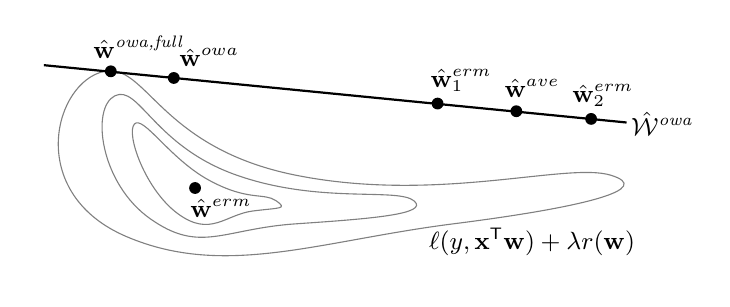
\begin{tikzpicture}
    [
    dot/.style = {minimum width=0.15cm,inner sep=0pt,line width=0pt,fill,circle,black,font=\small}
    , yscale=0.65
    ]
\small
\draw[gray] plot [smooth cycle,tension=1] coordinates {(-0.5,-0.75) (-1.05,1) (-0.1,-0.1) (0.75,-0.5) (0.45,-0.7) };
\draw[gray] plot [smooth cycle,tension=1] coordinates {(-0.85,-0.85) (-1.3,1.55) (0.25,0) (2.5,-0.5) (1,-0.95)};
\draw[gray] plot [smooth cycle,tension=1] coordinates {(-1.15,-1.2) (-1.5,2) (1,0) (5,0) (3,-0.95)};

\draw[thick] (-2.2,2.15) -- (5.2,1.03);

\node[dot] (wstar) at (-0.28,-0.25) {};
\node at (0.05,-0.65) {$\wmle$};

%\node[dot] (wstarproj) at (0.1,1.8) {};
%\draw (wstar) -- (wstarproj);
%\draw (0.07,1.65) -- (0.23,1.62) -- (0.26,1.78);

%\node[dot] (wavestar) at (4,0.5) {};
%\node                 at (4.5,0.3) {$\E\wave$};
\node[dot] (wave) at (3.8,1.25) {};
\node at (4.0,1.7) {$\wave$};
\node[dot] (wave) at (2.80,1.40) {};
\node at (3.1,1.85) {$\wmle_1$};
\node[dot] (wave) at (4.75,1.10) {};
\node at (4.9,1.55) {$\wmle_2$};
%\node[dot] (wave) at (3.8,1.25) {};

\node[dot] at (-1.35,2.03) {};
\node at (-1.0,2.5) {$\wowafull$};

\node[dot] at (-0.55,1.9) {};
\node at (-0.1,2.3) {$\wowa$};

\node at (4,-1.3) {$\loss(y,\trans\x\w)+\lambda \reg(\w)$};
\node at (5.65,1.0) {$\Wowa$};
\end{tikzpicture}
\vspace{-0.35in}
\caption{
    OWA performs a second optimization to find the best parameter vector in $\Wowa$.
    Since $\Wowa$ has low dimension, this optimization needs relatively little data to ensure that with high probability $\wowa$ has lower empirical loss than $\wave$.
}
\label{fig:contour}
\end{figure}

\subsection{The OWA Estimator}

Calculating the weights $\vfull$ directly is infeasible because it requires access to the full dataset.
Fortunately, we do not need to consider all the data points for an accurate estimator.
The parameter space $\Wowa$ is $m$-dimensional.
So intuitively, we only need $O(m)$ data points to solve the second optimization to our desired accuracy.
This intuition motivates the OWA estimator.
Let $\Zowa_i\subset Z_i$ be a set of $\nowa$ data points uniformly sampled from $Z_i$ without replacement,
and let $\Zowa$ be the union of the $\Zowa_i$s.
Then the OWA estimator is defined as
\begin{equation}
\label{eq:wowa}
\wowa = \matW \vowa,
\end{equation}
where
\begin{equation}
\label{eq:ahat}
\vowa = \argmax_{\vv\in\mathbb R^m} \sum _{(\x,y)\in \Zowa} \loss\left(y,\trans\x \matW \vv \right)
+ \lambda \reg(\matW\vv)
.
\end{equation}

We present two algorithms for calculating $\wowa$.
Algorithm \ref{fig:alg1} uses only a single round of communication, 
but requires that a predesignated master machine already have a copy of the $\Zowa$ dataset.
In the only round, each machine calculates $\wmle_i$ independently,
then transfers the result to the master.
A total of $O(dm)$ bits are transfered to the server.
(The parameter vector has $d$ dimensions and there are $m$ machines.)
The averaging estimator transfers the same information,
and so has the same $O(dm)$ communication complexity.
The only difference between the two algorithms is the way the master machine merges the local estimates.

If the master machine does not already have a copy of $\Zowa$,
then we must transfer a copy to the master. 
Algorithm \ref{fig:alg2} exploits the structure of the $\wowa$ estimator to transmit this data efficiently.
In the first round, each machine calculates $\wmle_i$ independently.
The result is then broadcast to every other machine, instead of just the master.
A total of $O(dm^2)$ bits are transmitted in this round.
(The parameter vector has $d$ dimensions,
there are $m$ machines,
and each machine transmits to each other machine.)
In the second round, each machine projects its local dataset $\Zowa_i$ onto the space $\Wowa$.
These projected data points are then transmitted to the master.
A total of $O(m^2\nowa)$ bits are transmitted.
(The projected data points each have dimension $m$, 
there are $m$ machines,
and there are $\nowa$ data points per machine.)
%The master machine now has all of the information to complete the optimization.
Theorem $\ref{theorem:wowa}$ suggests that $\nowa$ should be set to $O(mn/d)$.
So the total data transmitted in both rounds is $O(dm^2 + m^3n/d)$. 

%The communication complexity of Algorithm 1 is asymptotically worse than the averaging estimator, 
%which transmits only $O(dm)$ bits.
%But we claim this is not a problem for two reasons.
%First, this worse dependence on $m$ is not significant in practice because $m$ is much smaller than $n$ and $d$.
%We show in our experiments that when the problem is large enough to take a full day to solve for the $\wmle_i$s on the first round, the second round takes only several minutes.
%Second, with a slight modification to the problem setting, we can reduce the communication complexity to match the $O(dm)$ bound of the averaging estimator.
%In the original problem setting, we assume that the data points have already been communicated to the machines. 
%In particular, the $O(dm)$
%
%so whenever $d>m^2$ and $d>mn/d$, OWA has the same asymptotic communication complexity as averaging.
%When $d<m\nowa$, this is the same order of bits as the averaging estimator.


\begin{algorithm}[t]
\caption{Calculating $\wowa$ in one round}
\label{alg:distributed}
\begin{algorithmic}
\STATE Preconditions: 
\STATE ~~~~~each machine $i$ already has dataset $Z_i$
\STATE ~~~~~the master machine additionally has $\Zowa$
\STATE Round 1, each machine $i$ independently:
\STATE ~~~~~calculates $\wmle_i$ using \eqref{eq:wmlei}
\STATE ~~~~~transmits $\wmle_i$ to the master
\STATE The master calculates $\wowa$ using \eqref{eq:wowa} and \eqref{eq:ahat}
\end{algorithmic}
\label{fig:alg1}
\end{algorithm}


\begin{algorithm}[t]
\caption{Calculating $\wowa$ in two rounds}
\label{alg:distributed}
\begin{algorithmic}
\STATE Preconditions:
\STATE ~~~~~each machine $i$ already has dataset $Z_i$
\STATE Round 1, each machine $i$ independently:
\STATE ~~~~~calculates $\wmle_i$ using \eqref{eq:wmlei}
\STATE ~~~~~broadcasts $\wmle_i$ to all other machines
\STATE Round 2, each machine $i$ independently:
\STATE ~~~~~constructs $\matW=(\wmle_1,...,\wmle_m)$
\STATE ~~~~~samples a dataset $\Zowa_i\subset Z_i$ of size $\nowa$
\STATE ~~~~~calculates $\Zproj_i=\{(\trans\x\matW,y) : (\x,y)\in\Zowa\}$
\STATE ~~~~~sends $\Zproj_i$ to a master machine
\STATE The master calculates $\wowa$ using \eqref{eq:wowa} and \eqref{eq:ahat}
\end{algorithmic}
\label{fig:alg2}
\end{algorithm}

\subsection{Implementing with Existing Optimizers}
\label{sec:lambda2}

Equations \ref{eq:vfull} and \ref{eq:ahat} cannot be solved directly using off the shelf optimizers because existing optimizers do not support the non-standard regularization term $\reg(\matW\vv)$.
%This regularization is in principle no more difficult to optimize than the term $\reg(\w)$ from Equation $\ref{eq:wmle}$;
%it is simply not implemented.
In practice, it is sufficient to approximate this term by L2 regularization directly on the $\vv$ vector:
\begin{equation}
\lambda \reg(\matW\vv) \approx \lambda_2 \ltwo{\vv}^2
,
\label{eq:approxreg}
\end{equation}
where $\lambda_2$ is a new hyperparameter.
We provide two justifications for this approximation:
\begin{enumerate}
\item
When we want the parameter vector $\w$ to be sparse 
(and so the regularizer $\reg$ is the L1 norm), 
we have no reason to believe that the $\vv$ vector should be sparse.
The desired sparsity is induced by the regularization when solving for $\wmle_i$s and maintained in any linear combination of the $\wmle_i$s.
\item
As the size of the dataset increases, the strength of the regularizer decreases.
In this second optimization, the dimensionality of the problem is small,
so it is easy to add more data to make the influence of the regularization negligible.
\end{enumerate}

The new $\lambda_2$ regularization parameter should be set by cross validation.
This will be a fast procedure, however, because there are only $m\nowa <\!\!< mn$ data points to optimize over,
they have dimensionality $m<\!\!<d$,
and the L2 regularized problem is much easier to solve than the L1 problem.
Furthermore, this cross validation can be computed locally on the master machine without any communication.
We demonstrate empirically in Section \ref{sec:exp} that the overhead of determining $\lambda_2$ is negligible.
%With this minor modification, our distributed estimator can be implemented using any existing optimizer.
%Our experimental results in Section \ref{sec:exp} use this modified version of $\hat\vv$.

\section{RELATED WORK}
\label{sec:relwork}

There are two main categories of related work:
alternative estimators,
and bounds on the communication complexity of distributed learning.

%OWA is the first communication-efficient algorithm to achieve the optimal $O(1/\sqrt{mn})$ error rate under general conditions.

%The existing literature on communication-efficient distributed estimation requires relatively complicated techniques.

\subsection{Alternative Estimators}
\label{sec:alt}
The simplest and most popular non-interactive estimator is the averaging estimator:
\begin{equation}
\wave = \frac{1}{m}\sum_{i=1}^m \wmle_i
.
\end{equation}
Previous analysis of $\wave$ makes a number of limiting assumptions.
\citet{mcdonald2009efficient} analyze $\wave$ in the special case of L2 regularized maximum entropy models.
They provide tail bounds on $\ltwo{\wstar-\wave}$, 
showing that the deviation $\ltwo{\E\wave-\wave}$ reduces as $O((mn)^{-1/2})$,
but that the bias $\ltwo{\wstar-\E\wave}$ reduces only as $O(n^{-1/2})$.
Their analysis uses a martingale technique that requires the radius of the dataset be independent of the size of the dataset.
This is a particularly limiting assumption as even the simple case of
normally-distributed data does not satisfy it.
\citet{zhang2012communication} provide a more general analysis showing that the mean squared error (MSE) $\E\ltwo{\wstar-\wave}{}^2$ decays as $O((mn)^{-1} + n^{-2})$.
This matches the optimal MSE of $\wmle$ whenever $m<n$.
Their analysis also requires a number of technical assumptions.
For example, they assume the parameter space $\W$ is bounded.
This assumption does not hold under the standard Bayesian interpretation of L2 regularization as a Gaussian prior of the parameter space.
They further make strong convexity and 8\emph{th} order smoothness assumptions which guarantee that $\wmle_i$ is a ``nearly unbiased estimator'' of $\wstar$.
Most recently, \citet{rosenblatt2016optimality} analyze $\wave$ in the asymptotic regime as the number of data points $n\to\infty$.
This analysis is more general than previous analyses, but it does not hold in the finite sample regime.
Our analysis of OWA in Section \ref{sec:anal} requires no assumptions of boundedness or convexity and holds in the finite sample regime.
%In Section \ref{sec:anal}, we provide a simple analysis of $\wave$ that relaxes these assumptions.
%In particular, our analysis does not require any quantities to be bounded or a convex loss.

Other research has focused on modifications to the $\wave$ estimator to reduce bias.
\citet{zinkevich2010parallelized} show that if the training sets partially overlap each other (instead of being disjoint), then the resulting estimator will have lower bias.
\citet{lee2015communication} and \citet{battey2015distributed} independently develop techniques for debiasing L1-regularized problems.
%The authors admit their analysis is ``highly technical.''
\citet{zhang2012communication} provide a debiasing technique that works for any estimator.
%also provide a bootstrap average estimator,
%which works as follows.
It works as follows.
Let $r\in(0,1)$, and $Z_i^r$ be a bootstrap sample of $Z_i$ of size $rn$.
Then the bootstrap average estimator is
\begin{equation}
\wboot = \frac{\wave-r\waver}{1-r}
,
\end{equation}
where
\begin{equation}
\begin{aligned}
\waver &= \frac{1}{m}\sum_{i=1}^m \wmler_i
,
\\
\wmler_i &= \argmax_\w \sum_{(\x,y)\in Z_i^r} \loss(y,\trans\x\w) + \lambda \reg(\w)
.
%\\
%,
%\\
%\wboot & = \frac{\wave-r\waver}{1-r}
%.
\end{aligned}
\end{equation}
The intuition behind this estimator is to use the bootstrap sample to directly estimate and correct for the bias.
This estimator enjoys a MSE that decays as $O((mn)^{-1}+n^{-3})$ under similar assumptions as their analysis of $\wave$.
There are two main limitations to $\wboot$.
First, the optimal value of $r$ is not obvious and setting the parameter requires cross validation on the entire data set.
Our proposed $\wowa$ estimator has a similar parameter $\lambda_2$ that needs tuning,
but this tuning happens on a small fraction of the data and always with the L2 regularizer.
So properly tuning $\lambda_2$ is more efficient than $r$.
Second, performing a bootstrap on an unbiased estimator increases the variance.
This means that $\wboot$ could perform worse than $\wave$ on unbiased estimators.
Our $\wowa$ estimator, in contrast, will perform at least as well as $\wave$ with high probability, as seen in Figure \ref{fig:contour}.
In Section \ref{sec:exp}, we show that our estimator has better empirical performance.

%An alternative definition of the $\wave$ estimator is
%\begin{equation}
%\wave = \argmin_\w \frac{1}{m}\sum_{i=1}^m \ltwo{\wmle_i-\w}^2
%\end{equation}
%It is easy to show that the two definitions are equivalent with standard calculus.

\citet{liu2014distributed} propose a more Bayesian approach inspired by \citet{merugu2003privacy}.
Instead of averaging the model's parameters,
they directly ``average the models'' with the following KL-average estimator:
\begin{equation}
\wkl = \argmin_{\w\in\W} \sum_{i=1}^m \kl[\bigg]{p(\cdot;\wmle_i)}{p(\cdot;\w)}
.
\end{equation}
The minimization is performed via a bootstrap sample from the smaller models.
This method has three main advantages.
First, it is robust to reparameterizations of the model.
Second, it is statistically optimal for the class of non-interactive optimization methods.
(We show in the next section that this optimality bound does not apply to our $\wowa$ estimator due to our semi-interactive setting.)
Third, this method is general enough to work for any model,
whereas our proposed OWA method works only for linear models.
The main downside of the KL-average is that the minimization has a prohibitively high computational cost.
Let $n^{kl}$ be the size of the bootstrap sample.
Then the original implementation's MSE shrinks as $O((mn)^{-1}+(nn^{kl})^{-1})$.
This implies that the bootstrap procedure requires as many samples as the original problem to get a MSE that shrinks at the same rate as the averaging estimator.
\citet{han2016bootstrap} provide a method to reduce this rate to $O((mn)^{-1}+(n^2n^{kl})^{-1})$ using control variates, but the procedure remains prohibitively expensive.
Their experiments show the procedure scaling only to datasets of size $mn\approx10^4$,
whereas our experiments involve a dataset of size $mn\approx10^8$.

Surprisingly, \citet{zhang2013divide} show that in the special case of kernel ridge regression,
a reduction in bias is not needed to have the MSE of $\wave$ decay at the optimal sequential rate.
By a careful choice of regularization parameter $\lambda$,
they cause $\wmle_i$ to have lower bias but higher variance,
so that the final estimate of $\wave$ has both reduced bias and variance.
%This suggests that once the proper regularization parameter is known,
%there is no need for a bias reduction at all.
This suggests that a merging procedure that reduces bias is not crucial to good performance if we set the regularization parameter correctly.
Typically there is a narrow range of good regularization parameters,
and finding a $\lambda$ in this range is expensive computationally.
We show experimentally in Section \ref{sec:exp} that our method has significantly reduced sensitivity to $\lambda$.
Therefore, it is computationally cheaper to find a good $\lambda$ for our method than for the other methods discussed in this section.

\subsection{Performance Bounds}
\label{sec:bounds}

Performance bounds come in two flavors: statistical and information theoretic.
On the statistical side, \citet{liu2014distributed} show that for any non-interactive distributed estimator $\what$,
the quantity $\ltwo{\what-\wmle}{}^2$ decays as $\Omega(\gamma^2 \I^{-1}/n^2)$.
Here $\gamma$ is the statistical curvature of the model and $\I$ is the Fisher information.
Furthermore, they show that their KL-averaging estimator $\wkl$ matches this bound.
One consequence of this bound is that no non-interactive learner can achieve the optimal $O(1/\sqrt{mn})$ error rate on models with nonzero statistical curvature.
The vast majority of models used in practice have nonzero curvature.
The only models with zero curvature are full exponential families.
OWA is able to ``break'' this bound and achieve optimal error rate because of its semi-interactive setting.
A crucial assumption of Liu and Ihler's analysis is that the merge function not depend on the data.

\citet{shamir2014fundamental}, \citet{zhang2013information}, and \citet{garg2014communication} all provide information theoretic lower bounds on the sample complexity of non-interactive learning problems.
As above, however, their results are not applicable in our semi-interactive setting.
\citet{braverman2015communication} provide a bound that applies in all distributed settings.
In particular, they show that the minimax optimal error rate for least squares regression requires $\Omega(m\cdot\min\{n,d\})$ bits of communication. 
%This dependence on $d$ remains even when the number of nonzero entries of $\wstar$ is much less than $d$.
This bound essentially matches the communication complexity of Algorithm 1. %where we have assumed the master already has access to $\Zowa$.
%There is one information theoretic lower bound that does apply to us.
%Let the true parameter vector $\wstar$ be $k$-sparse.
%That is, $\lzero{\wstar} \le k$.
%%Then \cite{zhang2013information} showed that at least $\Omega(mk/\log m)$ bits of communication are required in the non-interactive setting,
%%and \cite{garg2014communication} improved this lower bound to $\Omega(mk)$.
%Surprisingly, \citet{braverman2015communication} show that the minimax optimal error rate for least squares regression requires $\Omega(m\cdot\min\{n,d\})$ bits of communication (independent of $k$) independent of the setting.
%This is important because sparsity does not reduce the amount of communication required, and this bound does apply in our setting.
%Recall that the communication cost of OWA is $O(dm^2+m^2n/d)$, which is looser than the lower bound.

%%%%%%%%%%%%%%%%%%%%%%%%%%%%%%%%%%%%%%%%%%%%%%%%%%%%%%%%%%%%%%%%%%%%%%%%%%%%%%%%

\section{ANALYSIS}
\label{sec:anal}

In this section, we show that the statistical error $\ltwo{\wstar-\wowa}$ decreases at the rate $O(1/\sqrt{mn})$.
The proof is broken into two steps.
First we show that $\Wowa$ is a good subspace to optimize over in the sense that the distance between $\Wowa$ and $\wstar$ is small.
Then we show that $\wowa$ is a good parameter to choose within $\Wowa$.
%
Our analysis depends on estimators obeying the following mild condition.

\newtheorem*{sgt}{The Sub-Gaussian Tail (SGT) Condition}
\begin{sgt}
Let $\what$ be a linear estimator trained on $n$ data points of dimension $d$.
Let $t>0$.
Then, with probability at least $1-\exp(-t)$,
\begin{equation}
%\ltwo{\wstar-\what} \le O\left( \sqrt\frac {dt} {n} \right)
\ltwo{\wstar-\what} \le O\left( \sqrt{dt/n} \right)
.
\label{eq:sgt}
\end{equation}
\end{sgt}

%Sub-Gaussian distributions have recently become an important tool in the analysis of high dimensional statistics.
%\cite{vershynin2010introduction} provides an accessible tutorial of these results.

The SGT condition is known to hold in many situations of interest.
In the asymptotic regime when $n\to\infty$,
very strong results of this form have been known since the 1960s.
Chapter 7 of \citet{lehmann1999elements} provides an elementary introduction to this work.
Lehman proves an asymptotic version of the SGT requiring only that $\loss$ be three times differentiable and that the data points be i.i.d.

Similar results hold in the non-asymptotic case $n<\infty$.
The simplest results place distributional assumptions on the data.
For example, \citet{negahban2009unified} considers the case when the data points are sub-Gaussian, the likelihood satisfies a ``restricted strong convexity condition,'' and the regularizer is decomposable.
Their resulting theorems are actually much stronger than the SGT condition:
They prove that the dependence on the dimension $d$ in Equation \ref{eq:sgt} can be replaced by the number of non-zero elements in the optimal parameter vector $\wstar$.
For sparse models, this is a major improvement.
%\citet{sivakumar2015beyond} provides similar bounds when the data are only sub-exponential (which is more general than sub-Gaussian).
The strongest non-asymptotic results known to the authors are due to \citet{spokoiny2012parametricestimation}.
Spokoiny does not place any distributional assumption on the data,
captures sparsity information through dependence on the Fisher information,
and does not even require the data to be i.i.d.
Spokoiny's only assumption is that the empirical loss admit a local approximation via the ``bracketing device,''
which is a generalization of the Taylor expansion.

%The main idea of our analysis is to show that $\Wowa$ is a good subspace to optimize over.
%This idea is captured in the following lemma.

The following lemma is an easy consequence of the SGT condition.
It formalizes the key idea that $\Wowa$ is a good subspace to optimize over.

\begin{lemma}
\label{lemma:wwstar}
Assume the $\wmle_i$s satisfy the SGT condition.
Let $t>0$. 
Then with probability at least $1-\exp(-t)$,
\begin{equation}
\label{eq:wwstar}
\min_{\w\in\Wowa}\ltwo{\w-\wstar} \le O(\sqrt{dt/mn})
%\min_{\w\in\Wowa}\ltwo{\w-\wstar} \le \sigma\sqrt{\frac{v_{t/m}}{n}}
%\prob{\min_{\w\in\Wowa}\ltwo{\w-\wstar} \ge \sqrt{\frac{v_t}{n}} } \le \exp(-tm)
.
\end{equation}
\end{lemma}

\begin{proof}
Using independence of the $\wmle_i$s and the SGT condition, we have that
\begin{align}
%~~~~~~~~~~~~~&\!\!\!\!\!\!\!\!\!\!\!\!\!\!\!\!\!\!\!\!\!\!\!\!\!\!\!\!\!\!\!
&\prob{\min_{\w\in\Wowa} \ltwo{\w-\wstar} \le O(\sqrt{dt/mn})}
\\
\ge &
\prob{\min_{i=1...m} \ltwo{\wmle_i-\wstar} \le O(\sqrt{dt/mn})}
\\
=&
1-\prob{\min_{i=1...m} \ltwo{\wmle_i-\wstar} > O(\sqrt{dt/mn})}
\\
= &
1-\left(\prob{\ltwo{\wmle_1-\wstar} > O(\sqrt{dt/mn})}\right)^m
\\
= &
1-\left(1-\prob{\ltwo{\wmle_1-\wstar} \le O(\sqrt{dt/mn})}\right)^m
\\
\ge &
1-\big(1-(1-\exp(-t/m))\big)^m
\\
= &
1-\exp(-t)
\label{eq:lemres}
.
\end{align}
\end{proof}

Next, we introduce a smoothness condition that will connect the $\w$ minimizing \eqref{eq:wwstar} to $\wowafull$.

\newtheorem*{hess}{The Hessian Condition}
\begin{hess}
For any vector $\w$ satisfying $\ltwo{\w}\le\ltwo{\wstar-\wowafull}$, we have that
\begin{equation}
\label{eq:hessiancondition}
\qlo\ltwo{\w-\wstar}^2 \le \Loss(\w) - \Loss(\wstar) \le \qhi\ltwo{\w-\wstar}^2
\end{equation}
where $\Loss(\w) = \sum_{(\x,y)\in Z}\loss(y;\trans\x\w)+\lambda\reg(\w)$.
\end{hess}

This condition is somewhat easier to understand in the asymptotic regime as $n\to\infty$.
In this regime, we have that $\ltwo{\wstar-\wowafull}\to0$,
so \eqref{eq:hessiancondition} is equivalent to requiring that the condition number of the Hessian $\nabla^2\Loss(\wstar)$ be $\qhi/\qlo$.

%Our next theorem applies the Hessian Condition to Lemma \ref{lemma:wwstar} to the error of $\wowafull$.

%%%%%%%%%%%%%%%%%%%%%%%%%%%%%%%%%%%%%%%%

\begin{figure*}[t]
%\begin{tikzpicture}
%\begin{tabular}{ccc}
  %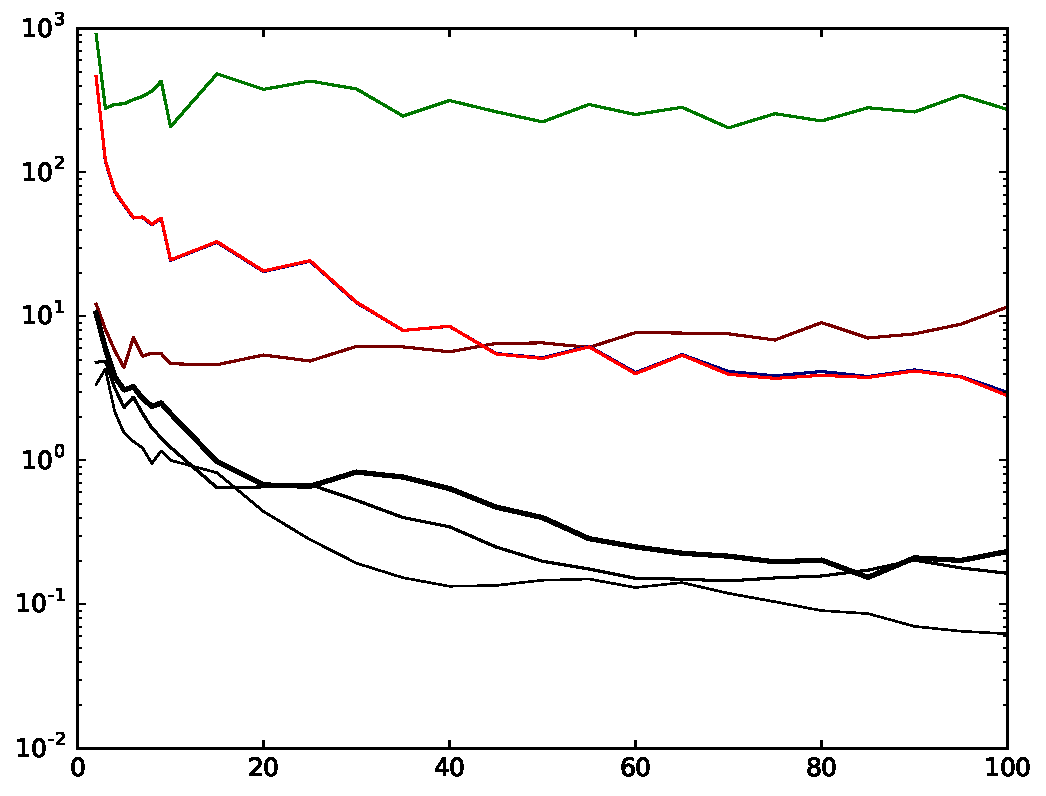
\includegraphics[width=0.3\textwidth]{img/logl2-auto-logl2-auto-normal-log-1000-100-star.pdf}
%& 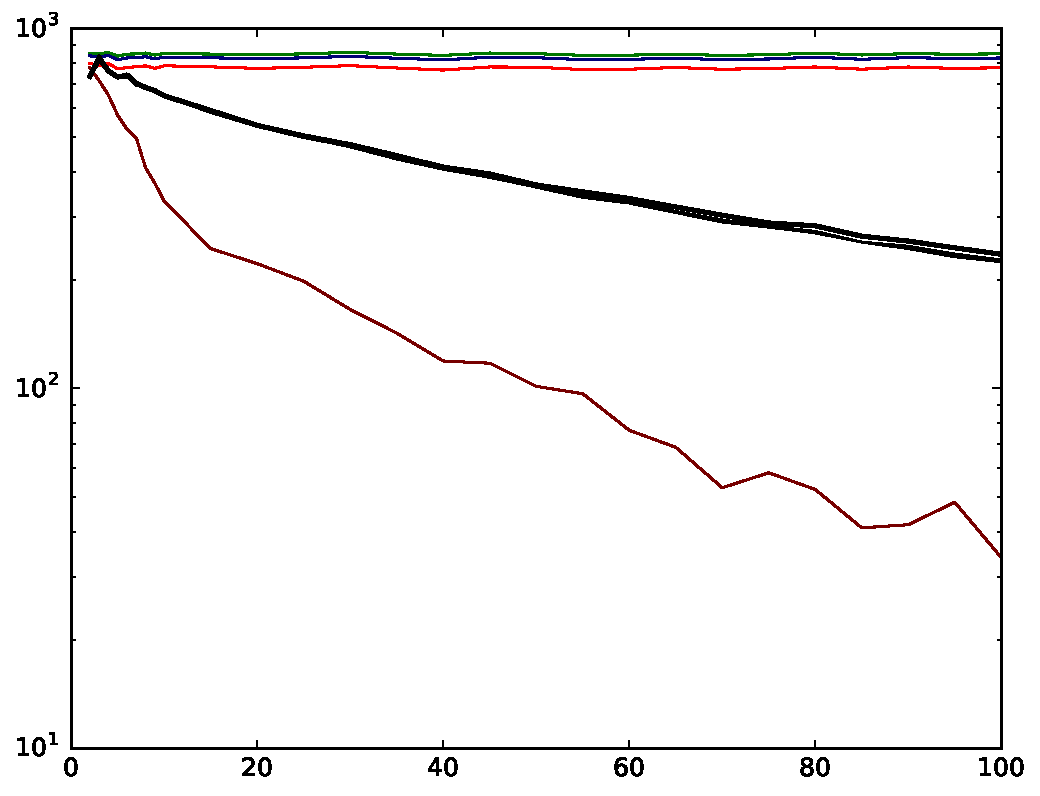
\includegraphics[width=0.3\textwidth]{img/logl2-auto-logl2-auto-normal-log-1000-1000-star.pdf}
%& 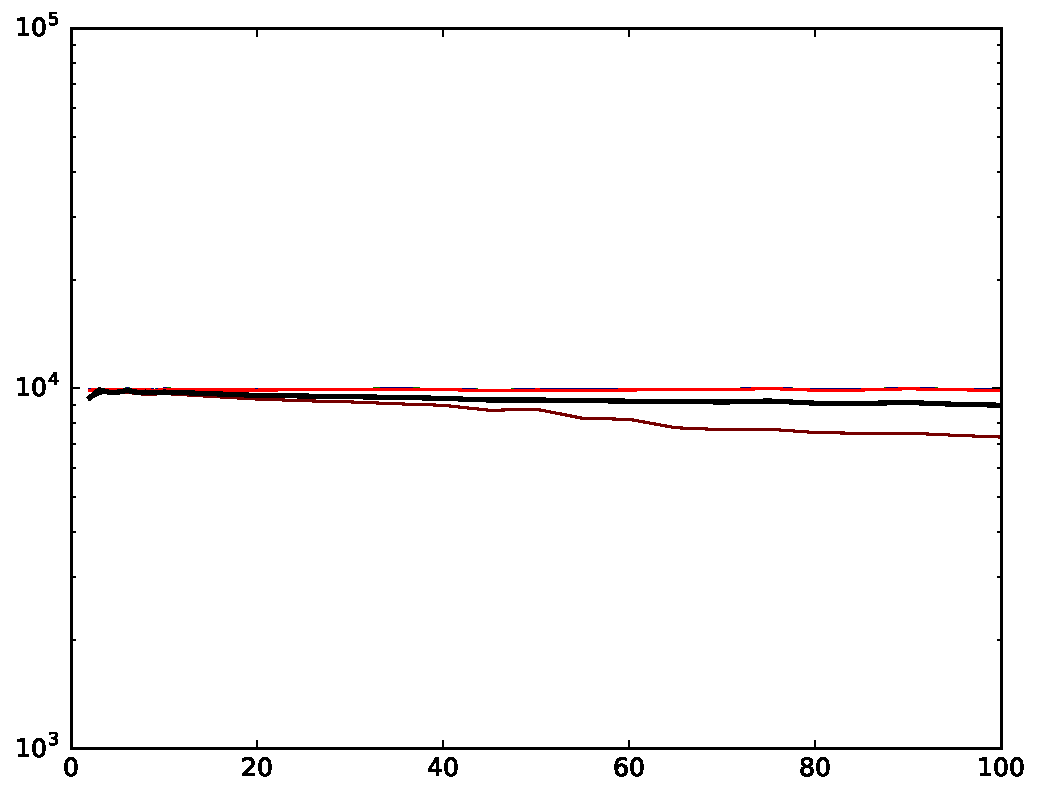
\includegraphics[width=0.3\textwidth]{img/logl2-auto-logl2-auto-normal-log-1000-10000-star.pdf}
%\\
  %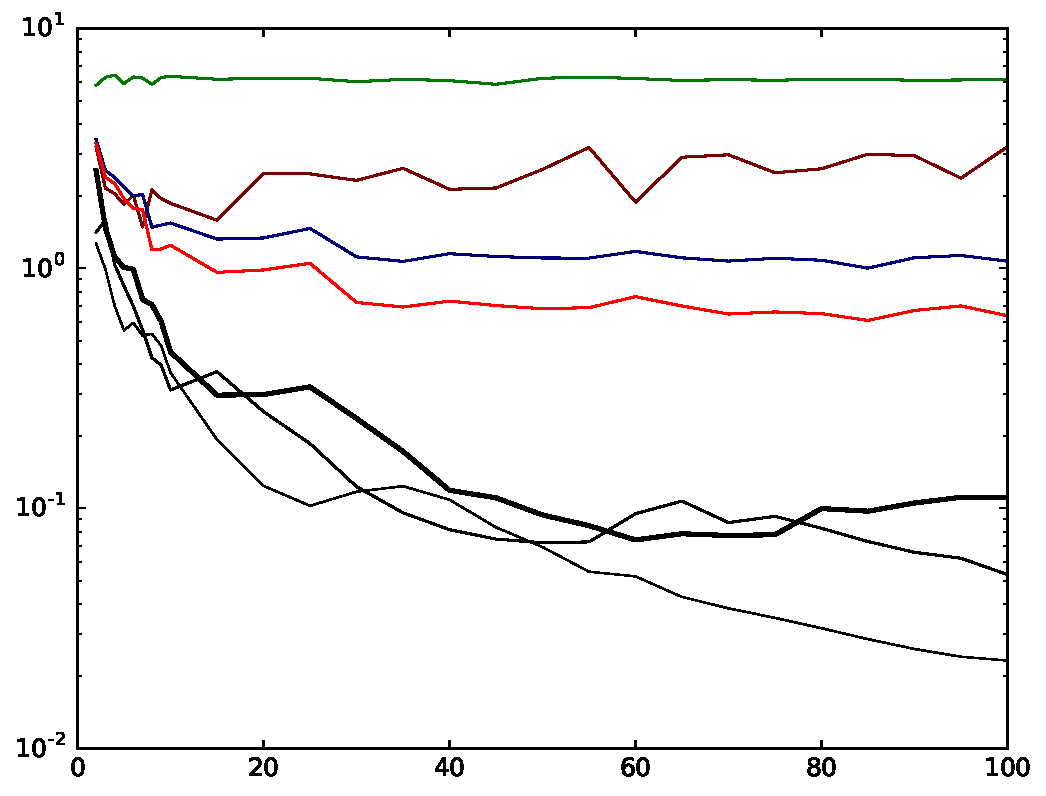
\includegraphics[width=0.3\textwidth]{img/logl2-auto-logl2-auto-uniform-log-1000-100-star.pdf}
%& 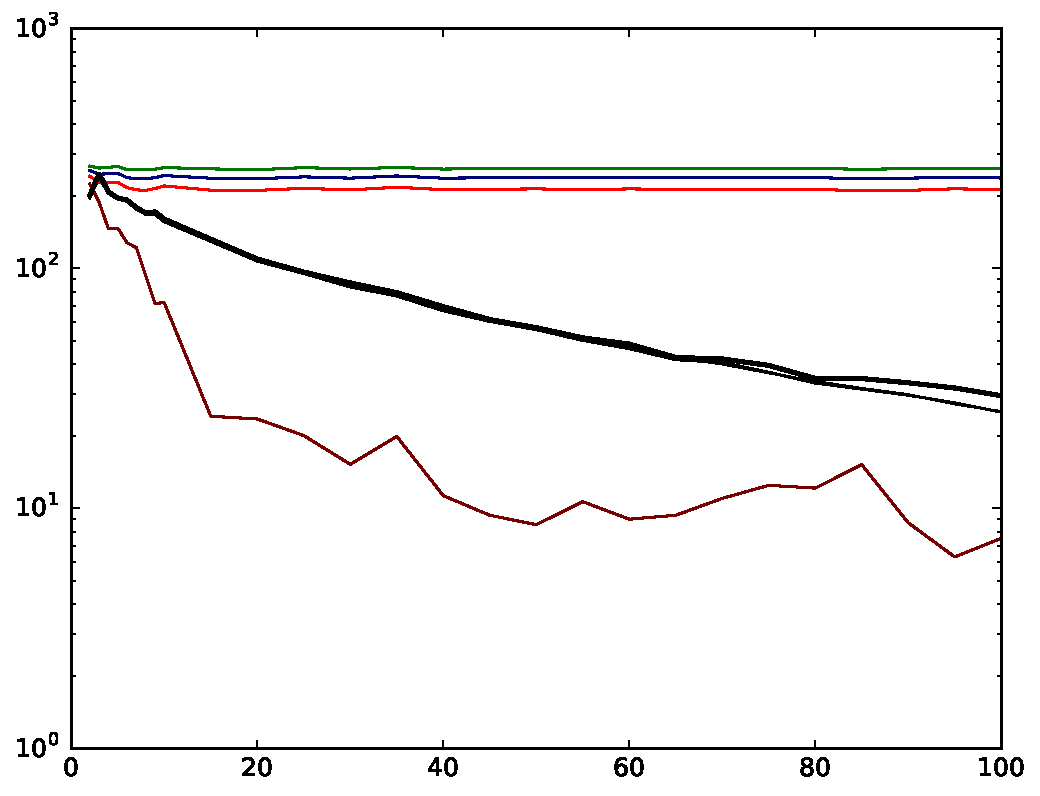
\includegraphics[width=0.3\textwidth]{img/logl2-auto-logl2-auto-uniform-log-1000-1000-star.pdf}
%& 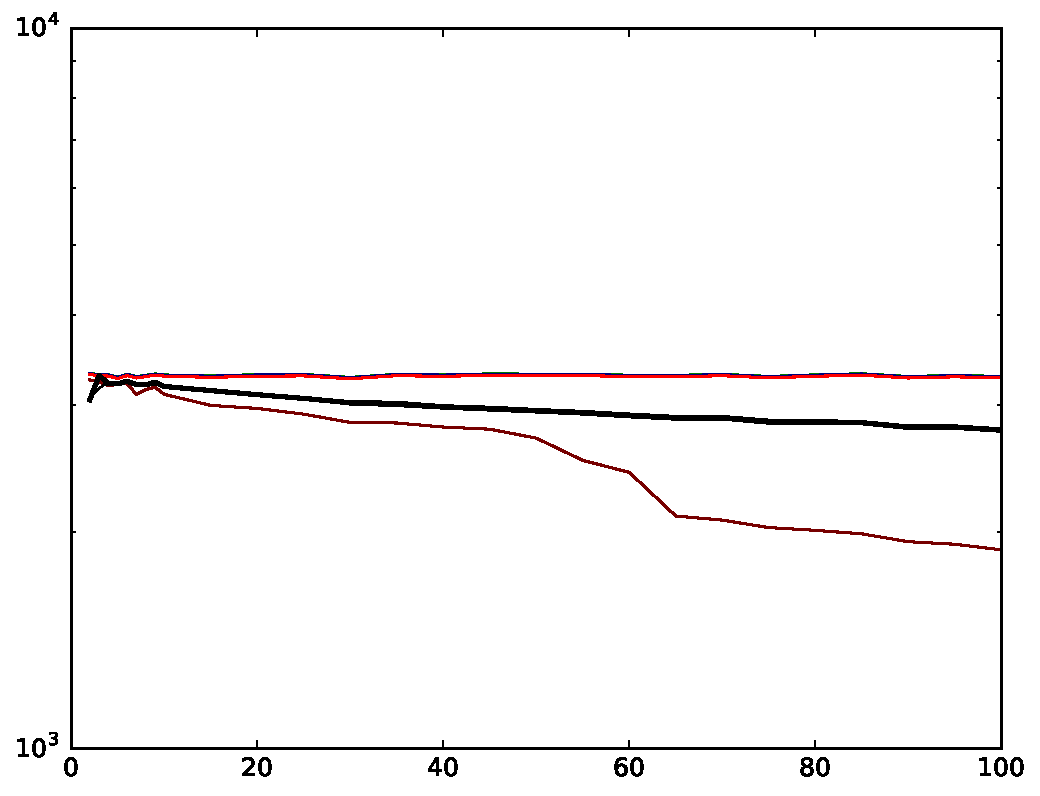
\includegraphics[width=0.3\textwidth]{img/logl2-auto-logl2-auto-uniform-log-1000-10000-star.pdf}
%\\
  %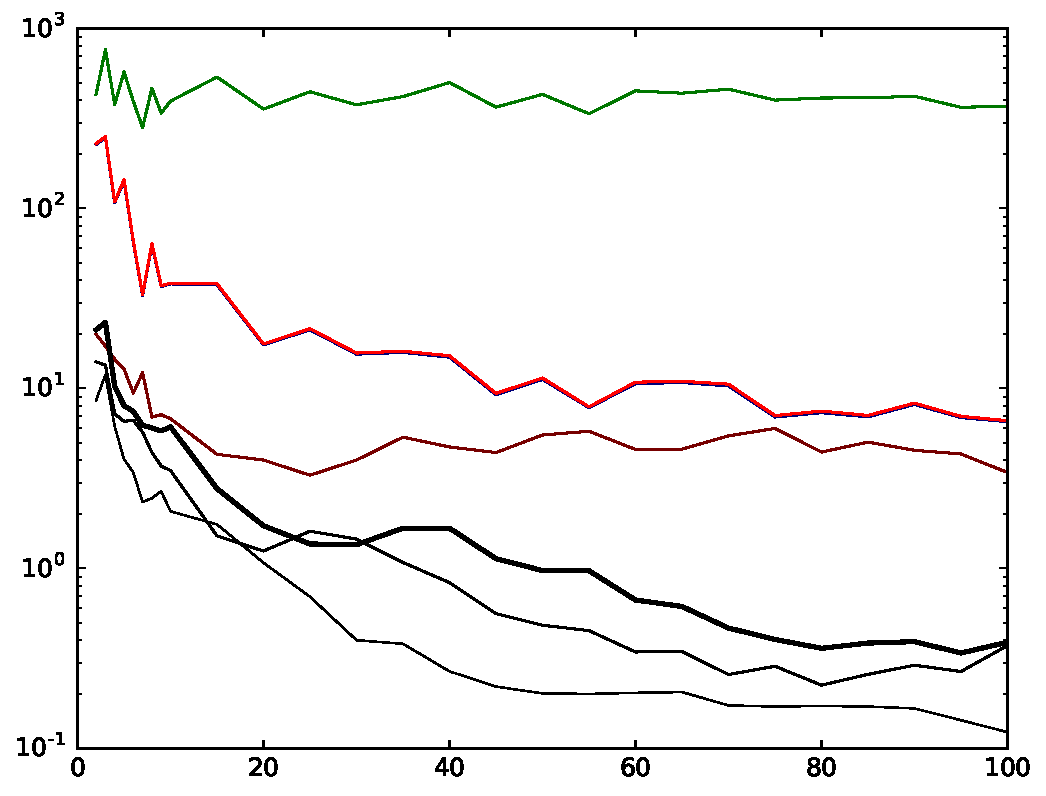
\includegraphics[width=0.3\textwidth]{img/logl1-auto-logl2-auto-laplace-log-1000-100-star.pdf}
%& 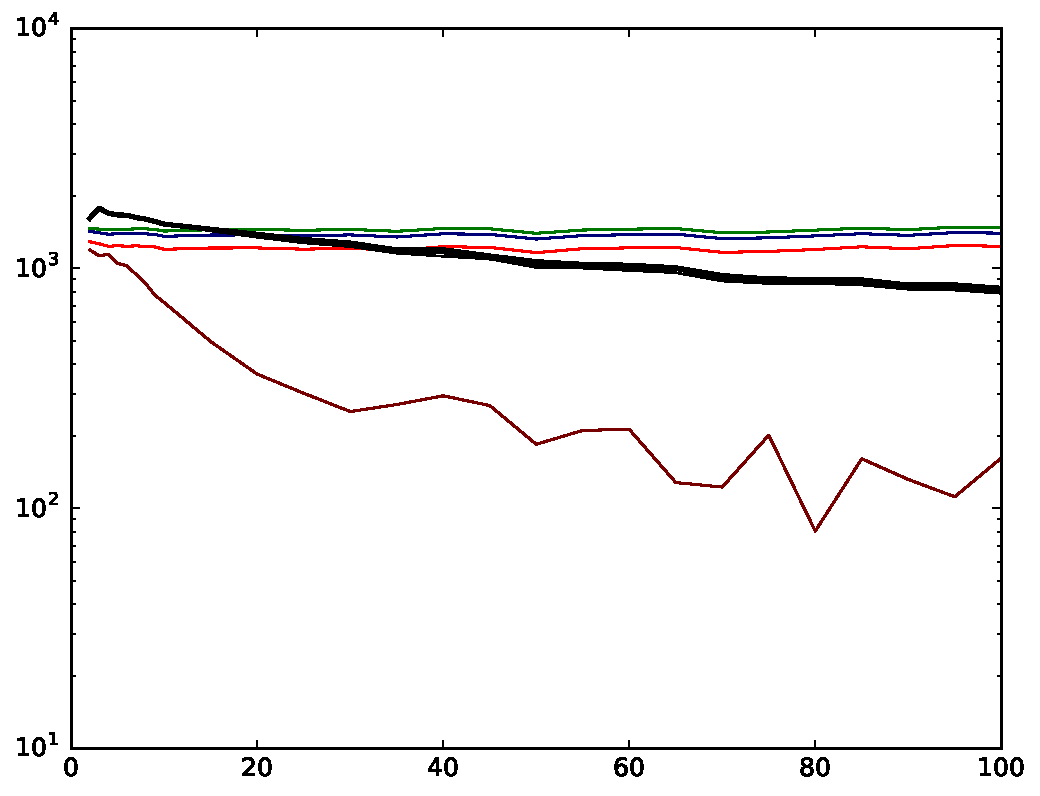
\includegraphics[width=0.3\textwidth]{img/logl1-auto-logl2-auto-laplace-log-1000-1000-star.pdf}
%& 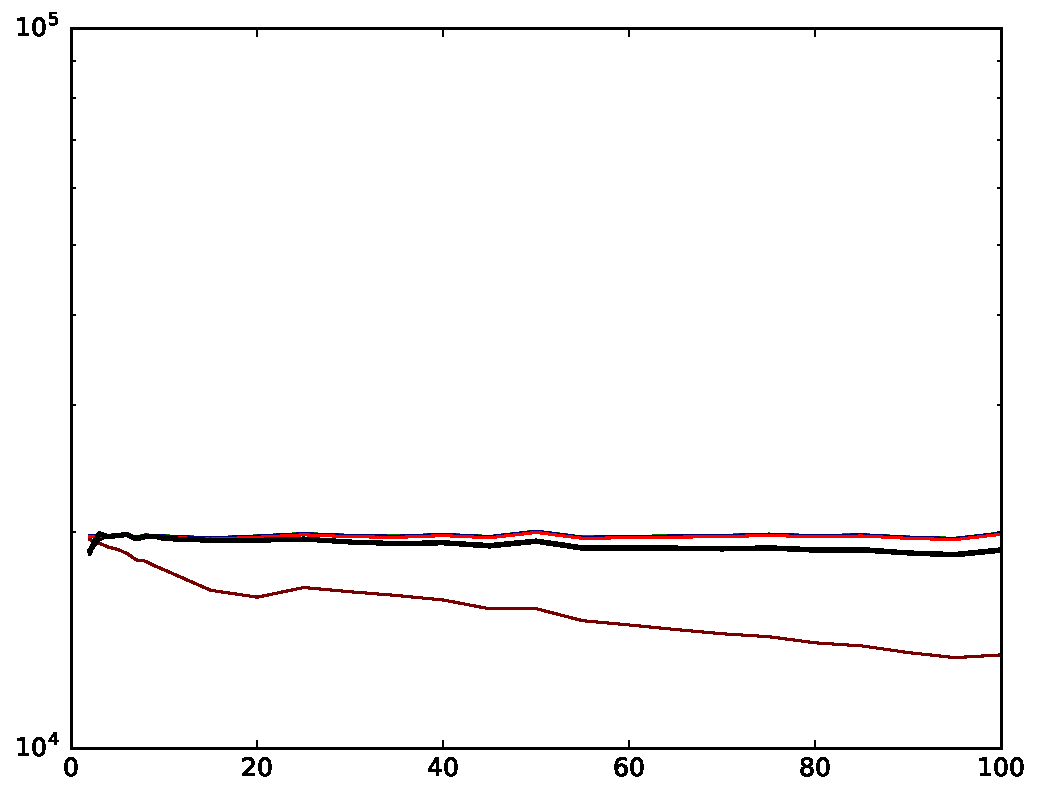
\includegraphics[width=0.3\textwidth]{img/logl1-auto-logl2-auto-laplace-log-1000-10000-star.pdf}
%\\
  %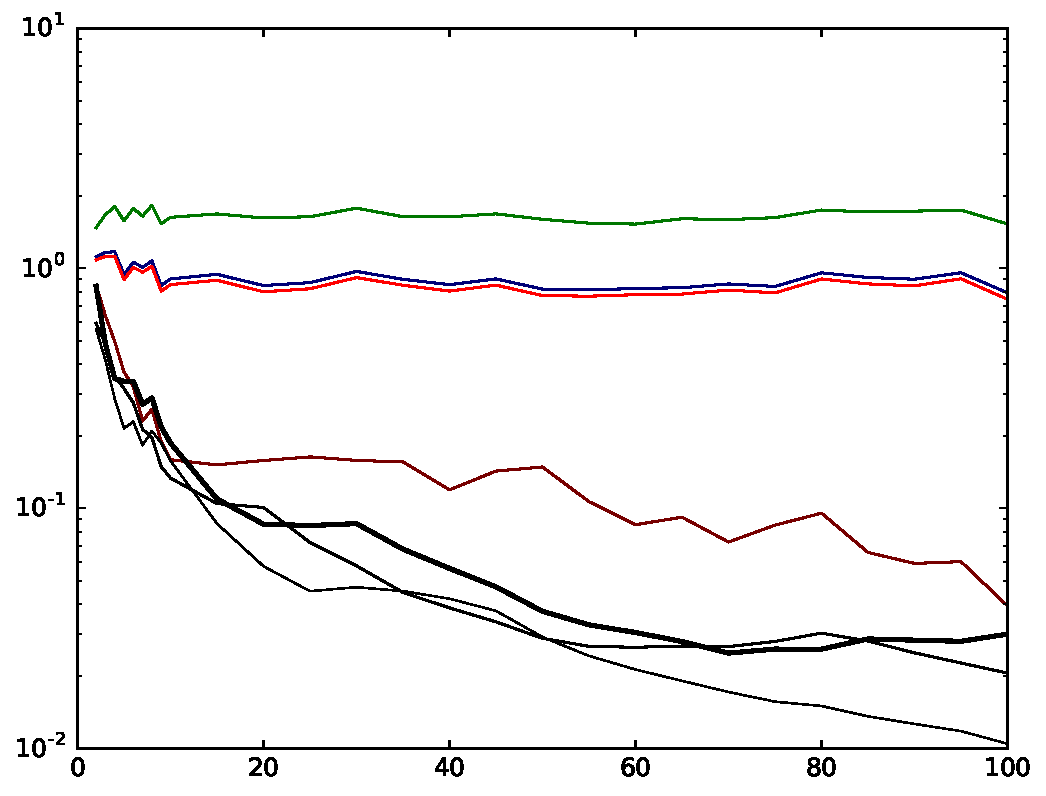
\includegraphics[width=0.3\textwidth]{img/logl1-auto-logl2-auto-spike-log-1000-100-star.pdf}
%& 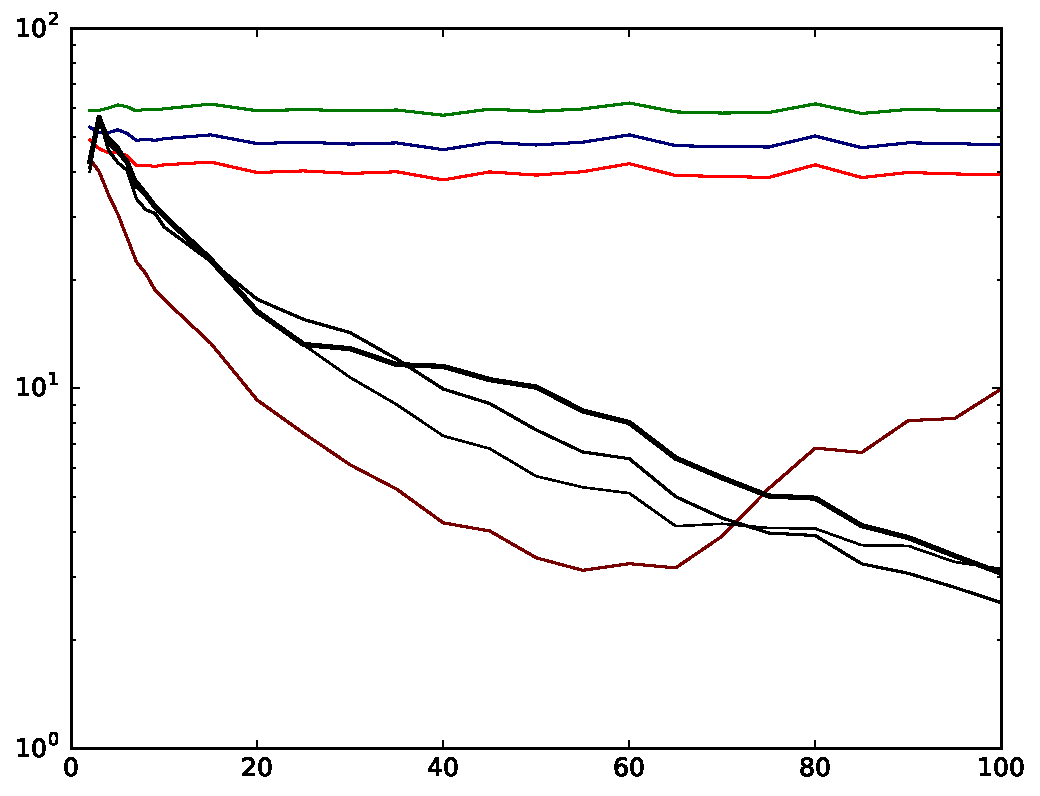
\includegraphics[width=0.3\textwidth]{img/logl1-auto-logl2-auto-spike-log-1000-1000-star.pdf}
%& 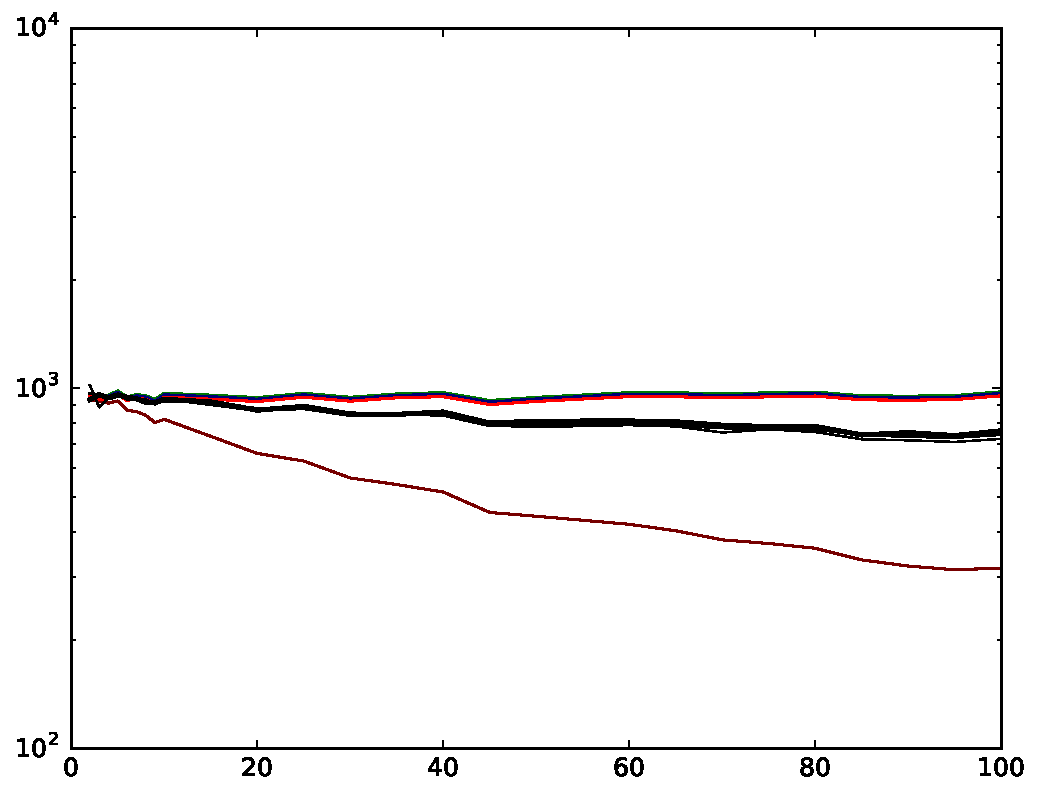
\includegraphics[width=0.3\textwidth]{img/logl1-auto-logl2-auto-spike-log-1000-10000-star.pdf}
%\end{tabular}
%\end{tikzpicture}
\plots{
\newcommand{\mklambdaplot}[4]{
\begin{tikzpicture}
    [ yscale=0.8
    ]
\tiny
#3
\begin{axis}
    [ width=0.35\textwidth
    %, xmode=log
    , ymode=log
    , xmin=1
    , xmax=100
#2
    ]
\addplot[black,no marks] table [x index=0,y index=5] {#1};
\addplot[brown,no marks] table [x index=0,y index=7] {#1};
\addplot[blue,no marks] table [x index=0,y index=9] {#1};
\addplot[red,thick,no marks] table [x index=0,y index=#4] {#1};
\addplot[darkgreen,very thick,no marks] table [x index=0,y index=55] {#1};
\addplot[dotted,darkgreen,very thick,no marks] table [x index=0,y index=56] {#1};
\addplot[darkgreen,very thin,no marks] table [x index=0,y index=56] {#1};
%\addplot[thick,red,no marks] table [x=n,y=bootll] {dat/kdd-scaling.dat};
%\addplot[very thick,darkgreen,no marks] table [x=n,y=owall] {dat/kdd-scaling.dat};
\end{axis}
\end{tikzpicture}
}
\begin{tabular}{cccc}
& $d=100$
& $d=1000$
& $d=10000$
\\
{\small\rotatebox{90}{\hspace{0.05cm}error $\ltwo{\wstar-\w}$}}
&\hspace{-0.5cm}\mklambdaplot
    {dat/logl1-auto-logl2-auto-spike-log-1000-100-star.pdf.csv}
    {,ymin=10^-2,ymax=10^1}
    { \node at (3,3) {\tiny\textcolor{brown}{$\wmle_i$}};
      \draw[->,brown] (2.7,2.85) -- (2.6,2.7);
      \node at (3.5,2.5) {\tiny\textcolor{blue}{$\wave$}};
      \draw[->,blue] (3.4,2.45) -- (3.45,2.35);
      \node at (2.5,1.9) {\tiny\textcolor{red}{$\wboot$}};
      \draw[->,thick,red] (2.5,2.0) -- (2.6,2.2);
      \node at (3.3,1.4) {\tiny$\wmle$};
      \draw[->] (3.2,1.3) -- (3.3,1.15);
      \node at (0.8,0.5) {\tiny\textcolor{darkgreen}{$\wowafull$}};
      \draw[->,darkgreen,dotted,thick] (0.8,0.65) -- (0.9,0.8);
      \draw[->,darkgreen,very thin] (0.8,0.65) -- (0.9,0.8);
      \node at (2.7,0.8) {\tiny\textcolor{darkgreen}{$\wowa$}};
      \draw[->,darkgreen,thick] (2.6,0.7) -- (2.7,0.55);
    }
    {19}
&\hspace{-0.5cm}\mklambdaplot
    {dat/logl1-autoreg-logl2-auto-spike-log-1000-1000-star.pdf.csv}
    {,ymin=10^0,ymax=10^2}
    {}
    {15}
&\hspace{-0.5cm}\mklambdaplot
    {dat/logl1-auto-logl2-auto-spike-log-1000-10000-star.pdf.csv}
    {}
    {}
    {11}
\\
& \hspace{0.2cm} {\small number of machines ($m$)}
&
&
\end{tabular}
}
\vspace{-0.15in}
\caption{
    In all three figures, the number of data points per machine is $m=1000$.
    Therefore, the left figure shows scalability in the low dimension regime,
    the middle figure in a medium dimension regime,
    and the right figure in a high dimension regime.
    $\wowa$ scales well with the number of machines in all cases.
    In particular, it scales with $m$ at the same rate as $\wmle$, whereas $\wave$ and $\wboot$ do not scale well with $m$ on this synthetic data.
    Surprisingly, $\wowa$ outperforms the oracle estimator trained on all of the data $\wmle$ in some situations.
    %This is likely due to the additional regularization introduced by the OWA algorithm,
    %as seen in Figure \ref{fig:lambda}.
    }
\label{fig:synscale}
\end{figure*}

%%%%%%%%%%%%%%%%%%%%%%%%%%%%%%%%%%%%%%%%

We are now ready to bound the error of $\wowafull$.

\begin{theorem}
\label{theorem:wowafull}
Assume the Hessian Condition and that the $\wmle_i$s satisfy the SGT condition.
Let $t>0$.
Then with probability at least $1-\exp(-t)$, 
\begin{equation}
%\ltwo{\wowafull-\wstar} \le \sqrt{\frac{\qhi}{\qlo}}\ltwo{\proj{\Wowa}\wstar}
%\ltwo{\wowafull-\wstar} \le \sqrt{\frac{\qhi}{\qlo}}\sqrt{\frac{v_t}{n}}
\ltwo{\wowafull-\wstar} \le O\left(
\sqrt{\bigg(\frac{\qhi}{\qlo}\bigg)\bigg(\frac{dt}{mn}\bigg)}
\right)
.
\end{equation}
\end{theorem}

\begin{proof}
Let $\proj{\Wowa}\wstar$ denote the vector in $\Wowa$ with minimum distance to $\wstar$.
That is, $\proj{\Wowa}\wstar$ is the vector minimizing \eqref{eq:wwstar}.
Then by the Hessian Condition, we have that
\begin{align}
\qlo\ltwo{\wowafull-\wstar}^2
&\le
\Loss(\wowafull) - \Loss(\wstar)
\\
&\le
\Loss(\proj{\Wowa}\wstar) - \Loss(\wstar)
\\
&\le
\qhi\ltwo{\proj{\Wowa}\wstar}^2
.
\end{align}
And so
\begin{equation}
\ltwo{\wowafull-\wstar} \le \sqrt{\frac{\qhi}{\qlo}}\ltwo{\proj{\Wowa}\wstar}
.
\end{equation}
The result follows by Lemma \ref{lemma:wwstar}.
\end{proof}



Next, we show that if $\nowa$ is set properly, then $\wowa$ and $\wowafull$ have the same error bounds.

\begin{theorem}
\label{theorem:wowa}
Assume the Hessian Condition and that both the $\wmle_i$s and $\vowa$ satisfy the SGT condition.
Let $\nowa=mn/d$ and $t>0$.
Then we have with probability at least $1-\exp(-t)$, 
\begin{equation}
\label{eq:wowathm}
\ltwo{\wowa-\wstar} \le 
O\left(
%\sqrt\frac{mt}{\nowa} 
%+
 \sqrt{\bigg(\frac{\qhi}{\qlo}\bigg)\bigg(\frac{dt}{mn}\bigg)}
 \right)
%\sqrt{\frac{v_t}{m\nowa}}
%+
%\sqrt{\bigg(\frac{\qhi}{\qlo}\bigg)\bigg(\frac{v_{t/m}}{n}\bigg)} 
\end{equation}
\end{theorem}

\begin{proof}
%Let $\wowastar$ be the vector in $\Wowa$ closest to $\wstar$.
We have by the triangle inequality that
\begin{equation}
\ltwo{\wowa-\wstar} 
\le 
\ltwo{\wowa-\wowafull} + \ltwo{\wowafull-\wstar}
\end{equation}
%\begin{align*}
%\ltwo{\wowa-\wstar} 
%&\le 
%\ltwo{\wowa-\wowastar} + \ltwo{\wowastar-\wstar}
%\\
%&\le 
%\ltwo{\wowa-\wowastar} + \ltwo{\wowafull-\wstar}
%.
%\end{align*}
Theorem \ref{theorem:wowafull} bounds the rightmost term above.
%Recall that the $\vv$ estimator in the second round 
Recall that the $\vowa$ estimator is trained on $m\nowa$ data points of dimension $m$ (see Equation \ref{eq:ahat}).
If we consider the true data distribution of this data to be the empirical distribution of sampling from $Z$, then the SGT condition for $\vowa$ states that
\begin{align}
\ltwo{\wowa-\wowafull} 
&\le O\left(\sqrt{mt/m\nowa}\right).
\\
&= O\left(\sqrt{t/\nowa}\right).
\end{align}
Substituting for $\nowa$ gives the desired result.
%and the SGT condition applied to $\vv$ bounds the left term.
%Notice that since $\vv$ is being optimized over a space of dimension $m$ instead of $d$,
%the $m$ appears in the numerator of the bound.
\end{proof}

%Some readers may object to Theorem \ref{theorem:wowa} above is that $\vv$ is unlikely to obey the SGT condition.

%%%%%%%%%%%%%%%%%%%%%%%%%%%%%%%%%%%%%%%%%%%%%%%%%%%%%%%%%%%%%%%%%%%%%%%%%%%%%%%%

\section{EXPERIMENTS}
\label{sec:exp}


We evaluate OWA on two logistic regression tasks.
The first task uses synthetic data.
The second task uses real world ad-click data from the Tencent search engine.
In each experiment, we compare $\wowa$ with four baseline estimators:
the naive estimator using the data from only a single machine $\wmle_i$;
the averaging estimator $\wave$;
the bootstrap estimator $\wboot$;
and the oracle estimator of all data trained on a single machine $\wmle$.
The $\wboot$ estimator has a parameter $r$ that needs to be tuned.
%We make an effort to present the $\wboot$ estimator in the best light possible.
In all experiments we evaluate $\wboot$ with $r \in \{0.005,0.01,0.02,0.04,0.1,0.2\}$,
which is a set recommended in the original paper \citep{zhang2012communication},
and then report only the value of $r$ with highest true likelihood.
Thus we are reporting an overly optimistic estimate of the performance of $\wboot$,
and as we shall see $\wowa$ still tends to perform better.

\begin{figure*}[t]
%\begin{tikzpicture}
%\node at (0,2) {};
%\node at (0,-2) {};
%\begin{tabular}{ccc}
  %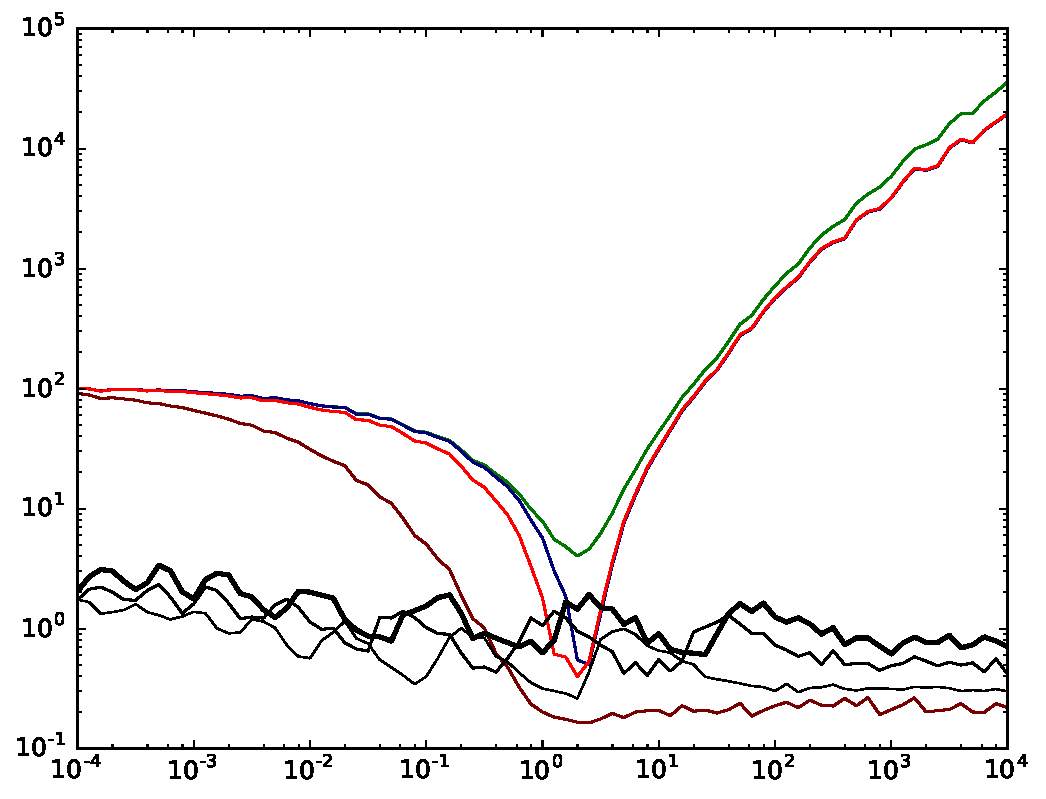
\includegraphics[width=0.3\textwidth]{img/logl2-star-logl2-auto-normal-log-1000-100-20}
%& 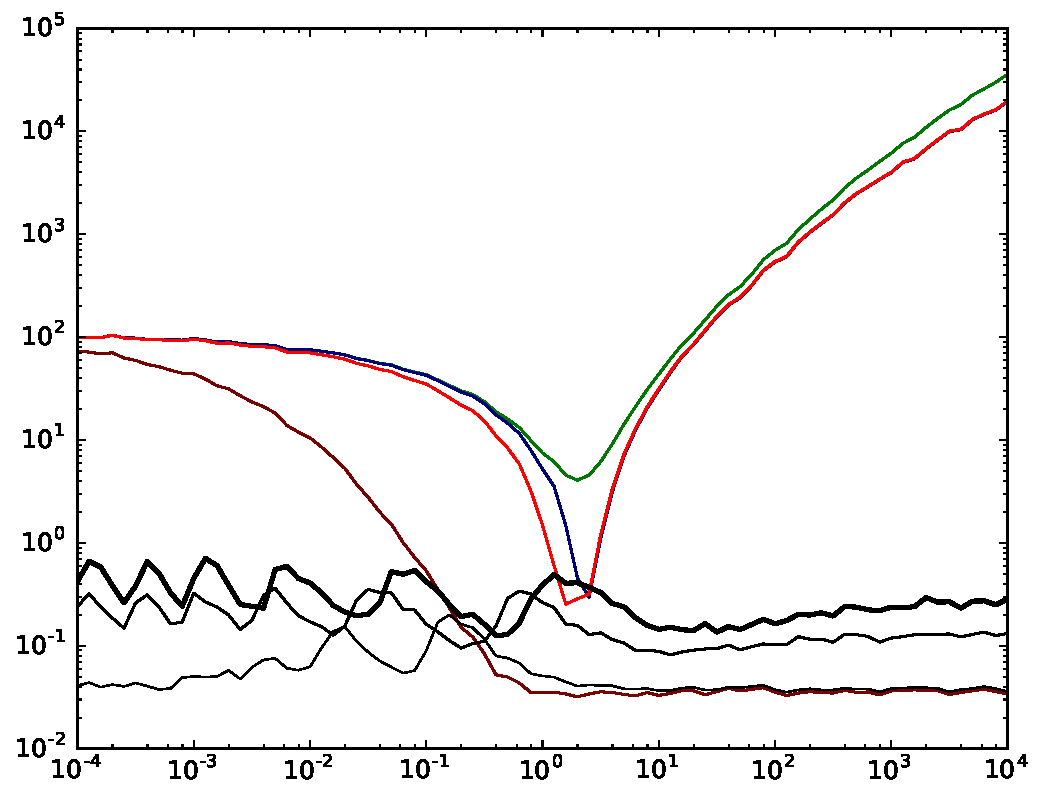
\includegraphics[width=0.3\textwidth]{img/logl2-star-logl2-auto-normal-log-1000-100-100}
%& 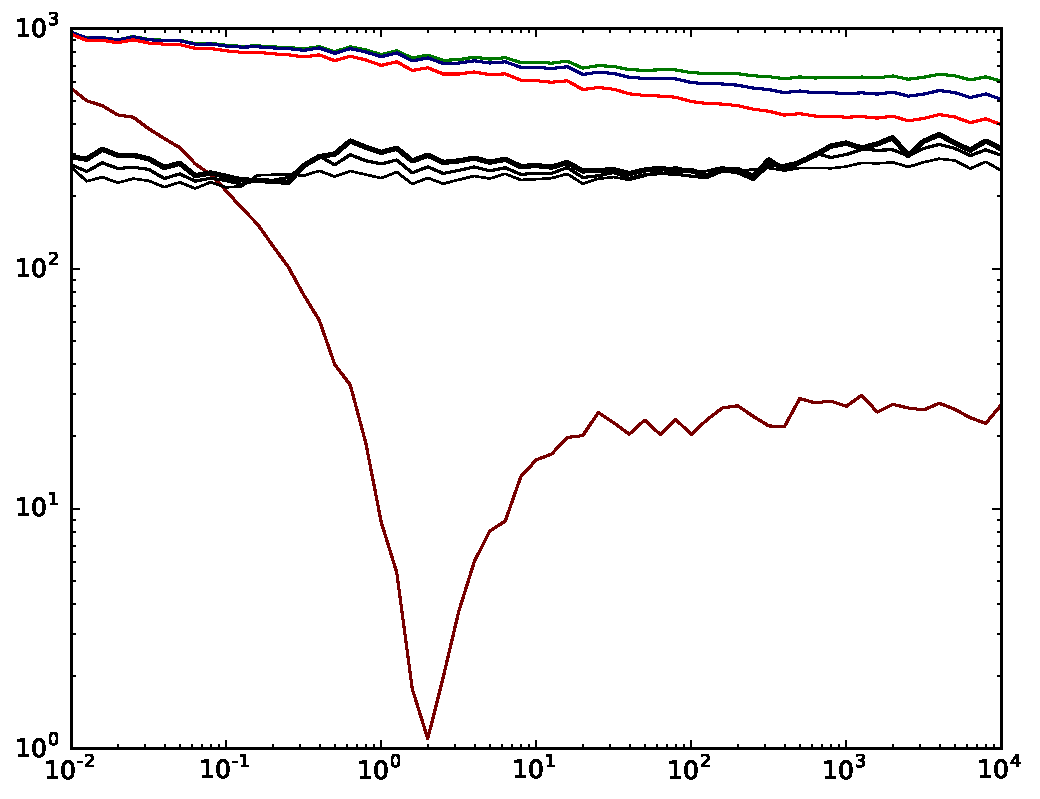
\includegraphics[width=0.3\textwidth]{img/logl2-star-logl2-auto-normal-log-1000-1000-100}
%\\
  %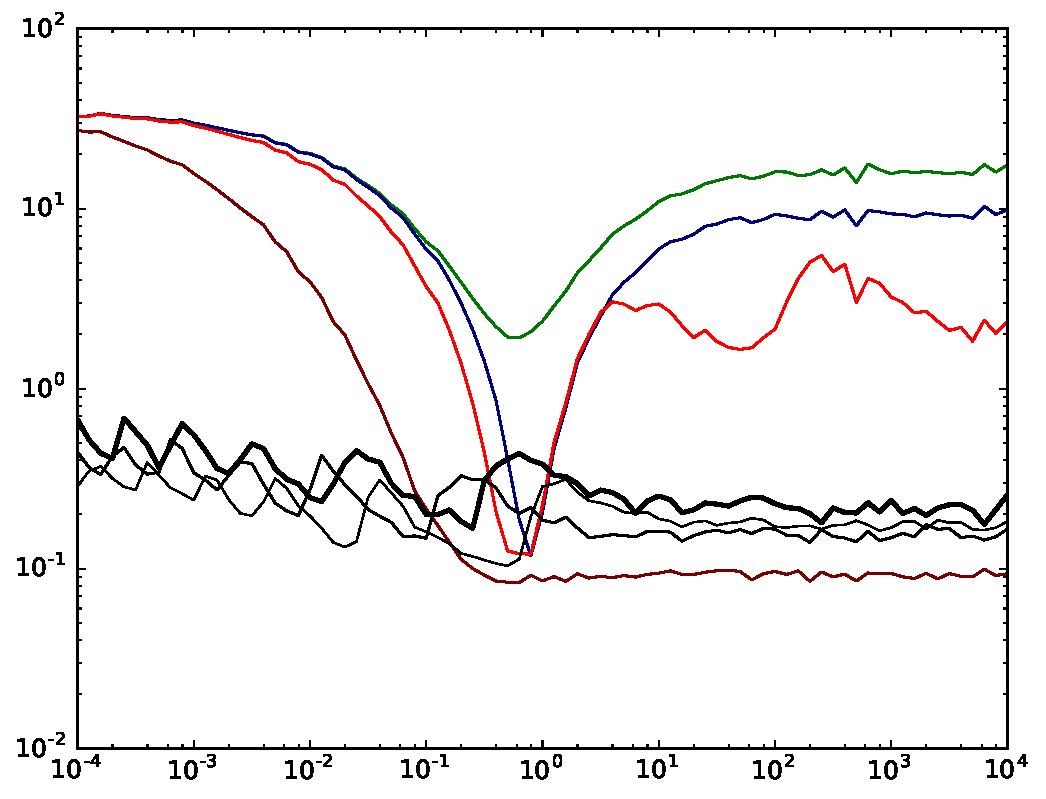
\includegraphics[width=0.3\textwidth]{img/logl2-star-logl2-auto-uniform-log-1000-100-20}
%& \includegraphics[width=0.3\textwidth]{img/logl2-star-logl2-auto-uniform-log-1000-100-100}
%& 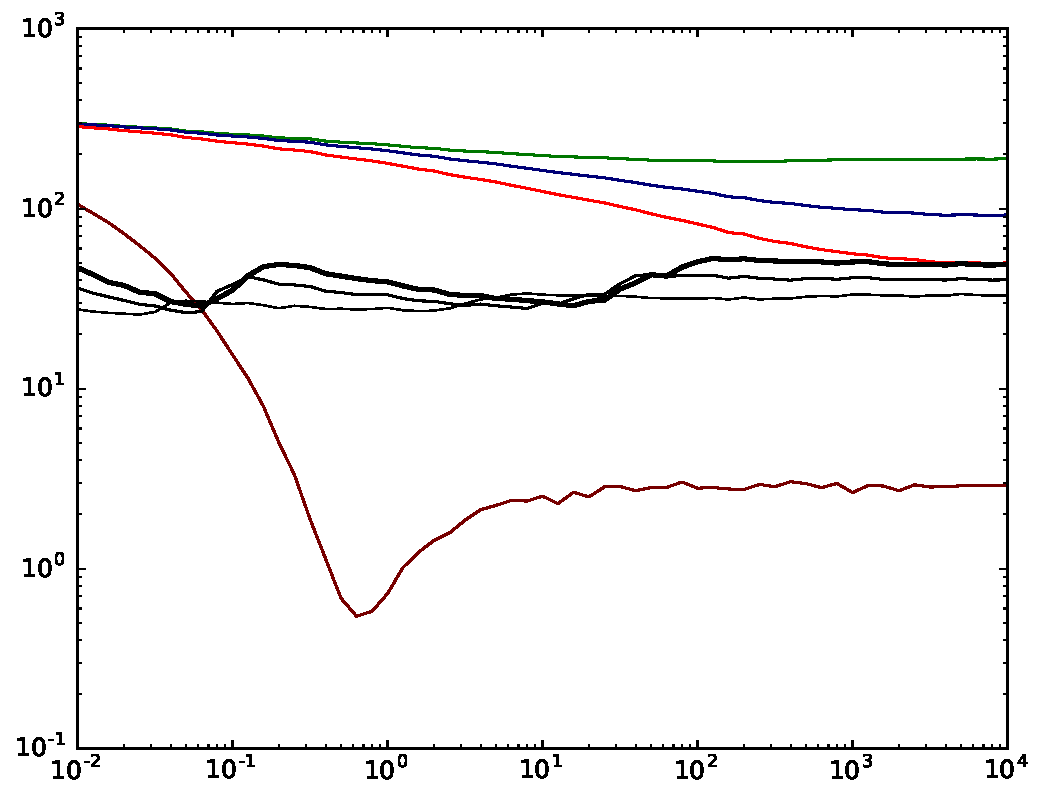
\includegraphics[width=0.3\textwidth]{img/logl2-star-logl2-auto-uniform-log-1000-1000-100}
%\\
  %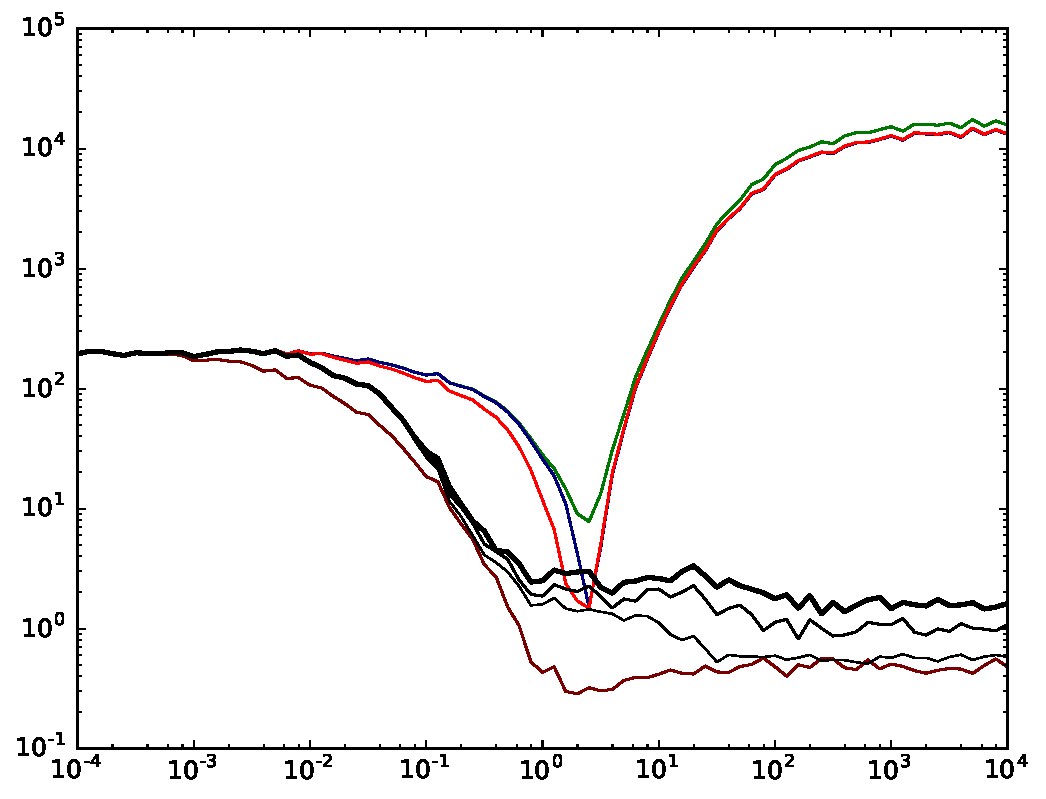
\includegraphics[width=0.3\textwidth]{img/logl1-star-logl2-autoreg-laplace-log-1000-100-20}
%& 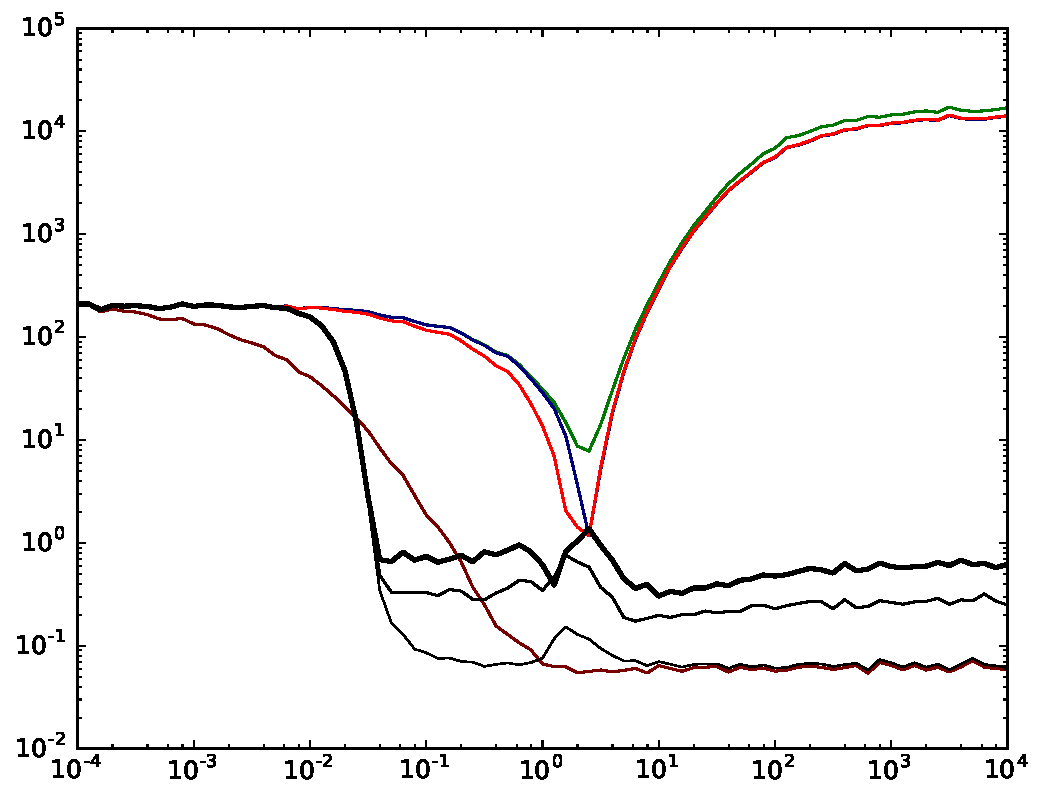
\includegraphics[width=0.3\textwidth]{img/logl1-star-logl2-auto-laplace-log-1000-100-100}
%& 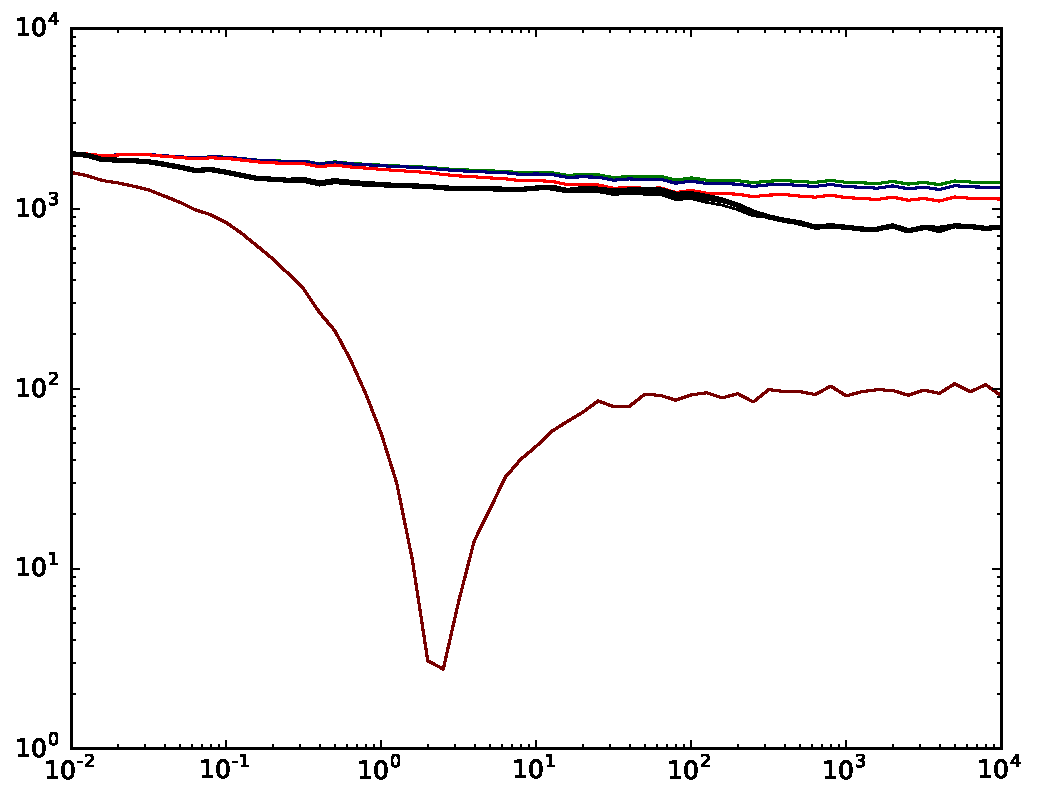
\includegraphics[width=0.3\textwidth]{img/logl1-star-logl2-auto-laplace-log-1000-1000-100}
%\\
  %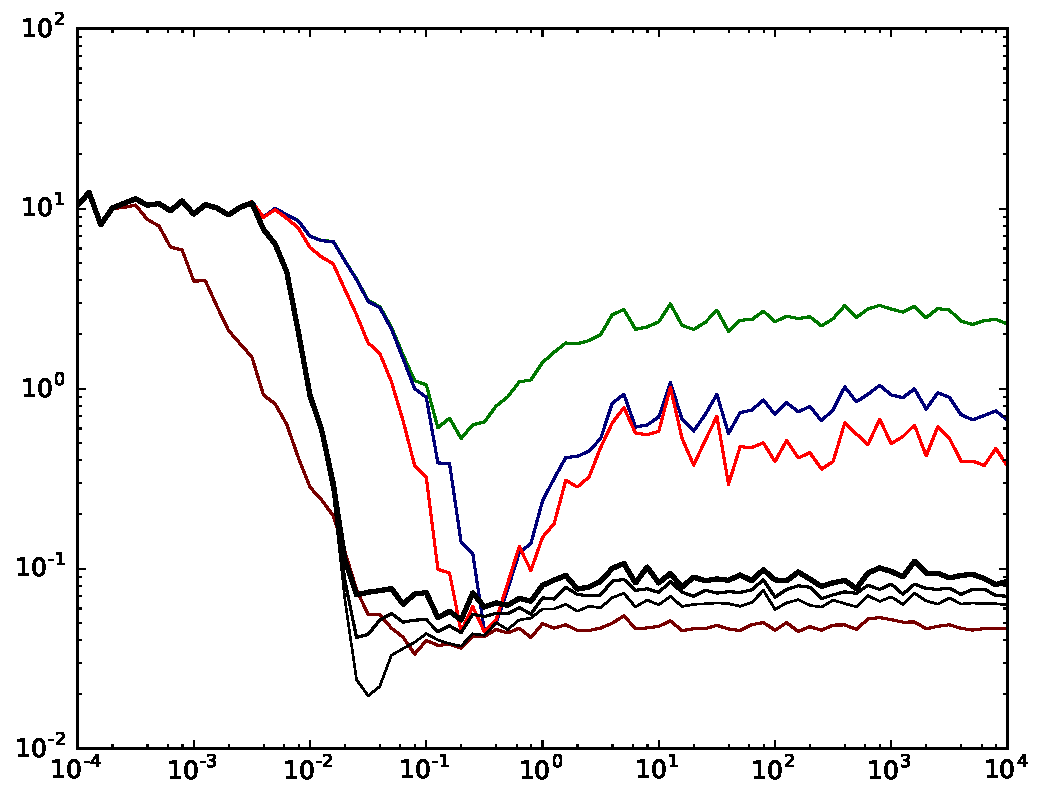
\includegraphics[width=0.3\textwidth]{img/logl1-star-logl2-autoreg-spike-log-1000-100-20}
%& 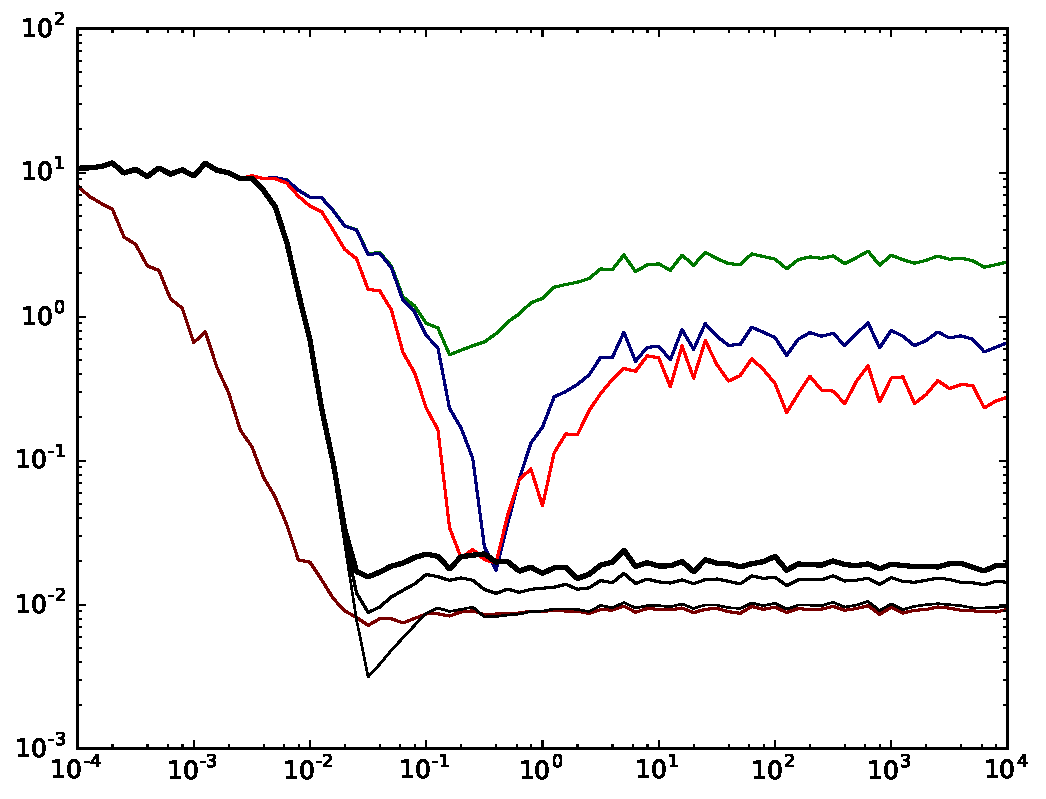
\includegraphics[width=0.3\textwidth]{img/logl1-star-logl2-auto-spike-log-1000-100-100}
%& 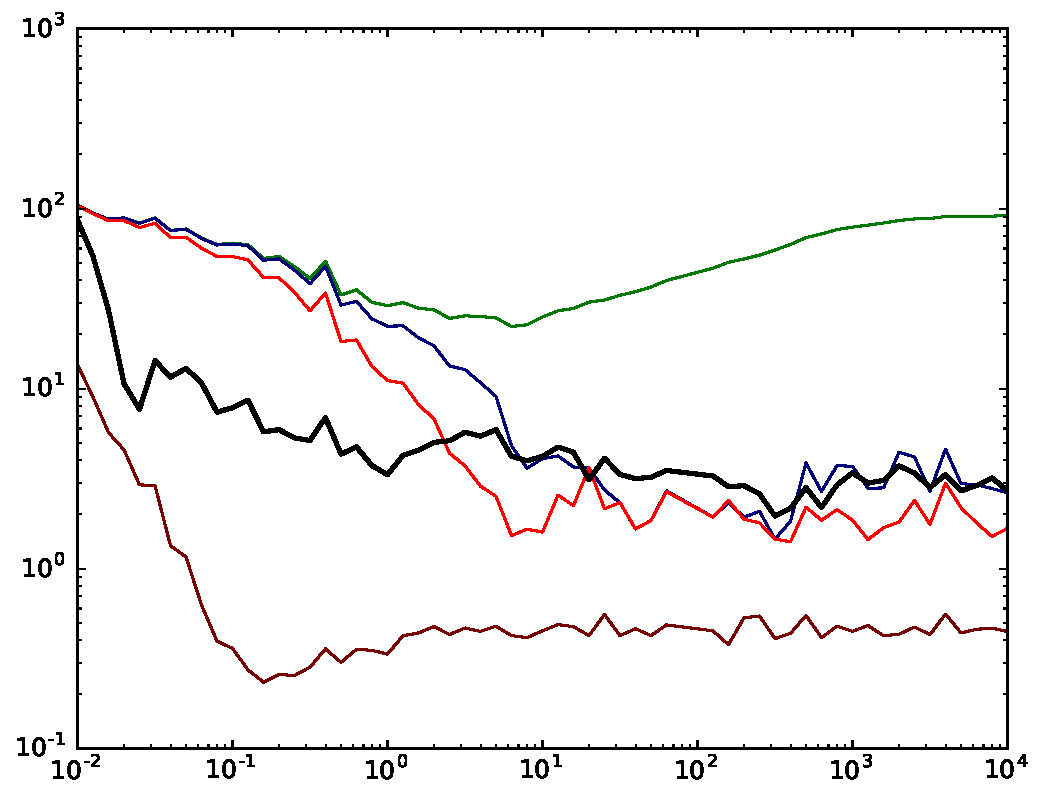
\includegraphics[width=0.3\textwidth]{img/logl1-star-logl2-auto-spike-log-1000-1000-100}
%\end{tabular}
%\end{tikzpicture}
\plots{
\newcommand{\mklambdaplot}[3]{
\begin{tikzpicture}
    [ yscale=0.8
    ]
\tiny
#3
\begin{axis}
    [ width=0.35\textwidth
    , xmode=log
    , ymode=log
    , xmin=10^-4
    , xmax=10^4
    , xtick={0.0001,0.01,1,100,10000}
    , enlarge y limits=0
#2
    ]
\addplot[black,no marks] table [x index=3,y index=5] {#1};
\addplot[brown,no marks] table [x index=3,y index=7] {#1};
\addplot[blue,no marks] table [x index=3,y index=9] {#1};
\addplot[red,thick,no marks] table [x index=3,y index=17] {#1};
\addplot[darkgreen,very thick,no marks] table [x index=3,y index=55] {#1};
\addplot[dotted,darkgreen,very thick,no marks] table [x index=3,y index=56] {#1};
\addplot[darkgreen,thin,no marks] table [x index=3,y index=56] {#1};
%\addplot[thick,red,no marks] table [x=n,y=bootll] {dat/kdd-scaling.dat};
%\addplot[very thick,darkgreen,no marks] table [x=n,y=owall] {dat/kdd-scaling.dat};
\end{axis}
%\node at (2.2,-0.8) {\small regularization strength ($\lambda$)};
\end{tikzpicture}
}
\begin{tabular}{cccc}
& $d=100,m=20$
& $d=100,m=100$
& $d=1000,m=100$
\\
{\small\rotatebox{90}{\hspace{0.05cm}error $\ltwo{\wstar-\w}$}}
&\hspace{-0.5cm}\mklambdaplot
    {dat.rev/logl1-star-logl2-autoreg-spike-log-1000-100-20.pdf.csv}
    {,ymin=10^-2,ymax=10^2,ytick={0.01,0.1,1,10,100}}{
    \node at (2,2.4) {\textcolor{brown}{$\wmle_i$}};
    \draw[->,brown] (2,2.3) -- (2.1,2);
    \node at (3.5,1.95) {\textcolor{blue}{$\wave$}};
    \draw[->,blue] (3.5,1.9) -- (3.55,1.75);
    \node at (4,1.1) {\textcolor{red}{$\wboot$}};
    \draw[->,thick,red] (3.8,1.3) -- (3.75,1.45);
    \node at (0.5,1.85) {$\wmle$};
    \draw[->] (0.5,2.0) -- (0.6,2.2);
    \node at (0.7,0.9) {\textcolor{darkgreen}{$\wowa$}};
    \draw[->,thick,darkgreen] (0.9,0.8) -- (1.2,0.8);
    \node at (0.6,0.4) {\textcolor{darkgreen}{$\wowafull$}};
    \draw[->,thick,dotted,darkgreen] (0.9,0.3) -- (1.2,0.3);
    \draw[->,very thin,darkgreen] (0.9,0.3) -- (1.2,0.3);
    }
&\hspace{-0.5cm}\mklambdaplot
    {dat.rev/logl1-star-logl2-auto-spike-log-1000-100-100.pdf.csv}
    {,ymin=10^-3,ymax=10^2,ytick={0.001,0.01,0.1,1,10,100}}
    {}
&\hspace{-0.5cm}\mklambdaplot
    {dat.rev/logl1-star-logl2-auto-spike-log-1000-1000-100.pdf.csv}
    {,ymin=10^-1,ymax=10^3,ytick={0.1,1,10,100,1000}}
    {}
\\
& \hspace{0.2cm} {\small regularization strength ($\lambda$)}
&
&
\end{tabular}
}
\caption{
    OWA is robust to the regularization strength.
    Surprisingly, additional regularization introduced by OWA lets it outperform the oracle estimator $\wmle$ in some cases.
    Our theory states that as $m\to d$, we have that $\Wowa\to\W$, and so $\wowa\to\wmle$.
    This is confirmed in the middle experiment.
    In the left experiment, $m<d$, but $\wowa$ still behaves similarly to $\wmle$.
    In the right experiment, $\wowa$ has similar performance as $\wave$ and $\wboot$ but is more robust to $\lambda$.
    }
\label{fig:lambda}
\end{figure*}

\subsection{Synthetic Data}

We generate the data according to the following sparse logistic regression model.
Each component of the true parameter vector $\wstar$ is sampled i.i.d.\ from a spike and slab distribution.
With probability 0.9, the component is 0;
with probability 0.1, the component is sampled from a standard normal distribution.
The data points are then sampled as
\begin{equation}
\begin{aligned}
\x_i &\sim \normal{0}{I}
,
~~~
y_i = \left(1+\exp(-\trans\x_i\wstar)\right)^{-1}
.
\end{aligned}
\end{equation}
The primary advantage of synthetic data is that we know the model's true parameter vector.
So for each estimator $\what$ that we evaluate, we can directly calculate the error $\ltwo{\what-\wstar}$.
We run two experiments on the synthetic data.
In both experiments, we use the L1 regularizer to induce sparsity in our estimates of $\wstar$.
Results are qualitatively similar when using a Laplace, Gaussian, or uniform prior on $\wstar$, and with L2 regularization.
%Our estimators will be biased because the model is misspecified.
%(L1 regularization corresponds to a Laplace prior on the parameter vector.)
%The true model for L1 regularization has a Laplace prior on $\wstar$.
%These results are not shown due to space limitations.

Our first experiment shows how the estimators scale as the number of machines $m$ increases.
We fix $n=1000$ data points per machine,
so the size of the dataset $mn$ grows as we add more machines.
This simulates the typical ``big data'' regime where data is abundant,
but processing resources are scarce.
For each value of $m$, we generate 50 datasets and report the average of the results.
Our $\wowa$ estimator was trained with $\nowa=128$.
The results are shown in Figure \ref{fig:synscale}.
As the analysis predicted, the performance of $\wowa$ scales much better than $\wave$ and $\wboot$.
Surprisingly, in the low dimensional regimes, $\wowa$ outperforms the single machine oracle $\wmle$.

One issue that has been overlooked in the literature on non-interactive distributed estimation is how to best set $\lambda$.
There are two natural ways to use cross validation and grid search.
The first is: for each $\lambda$ in the grid, perform the full training procedure including all communications and merges.
Then select the $\lambda$ with lowest cross validation error.
Unfortunately, this requires many rounds of communication (one for each $\lambda$ we are testing).
This extra communication largely negates the main advantage of non-interactive learners.
The second is: each machine independently uses cross validation to select the $\lambda$ that best fits the data locally when calculating $\wmle_i$.
In our experiments we use this second method due to three advantages.
First, there is no additional communication because model selection is a completely local task.
Second, existing optimizers have built-in model selection routines which make the process easy to implement.
We used the default model selection procedure from Python's SciKit-Learn \citep{scikit-learn}.
Third, the data may be best fit using different regularization strengths for each machine.
It is unclear which method previous literature used to select $\lambda$.
As mentioned in Section \ref{sec:lambda2}, OWA requires an additional round of cross validation during the master's merge procedure to set $\lambda_2$.
This cross validation is particularly fast and requires no communication with other machines.

Our second experiment shows the importance of proper $\lambda$ selection.
We evaluate the performance of the estimators with $\lambda$ varying from $10^{-4}$ to $10^4$ on a grid of 80 points.
Figure \ref{fig:lambda} shows the results. 
The $\wowa$ estimator is more robust to the choice of $\lambda$ than the other distributed estimators.
%Surprisingly, $\wowa$ even outperforms the oracle $\wmle$ in some regimes.
%This is likely due to additional regularization induced by the approximation in Equation \ref{eq:approxreg}.

\subsection{Real World Advertising Data}

We evaluate the estimators on real world data from the KDD 2012 Cup \citep{kddcup2012}.
The goal is to predict whether a user will click on an ad from the Tencent internet search engine.
This dataset was previously used to evaluate the performance of $\wboot$ \citep{zhang2012communication}.
This dataset is too large to fit on a single machine,
so we must use distributed estimators,
and we do not provide results of the oracle estimator $\wmle$ in our figures.
There are 235,582,879 distinct data points,
each of dimension 741,725.
The data points are sparse, so we use the L1 norm to encourage sparsity in our final solution.
The regularization strength was set using cross validation in the same manner as for the synthetic data.
For each test, we split the data into 80 percent training data and 20 percent test data.
The training data is further subdivided into 128 partitions,
one for each of the machines used.
It took about 1 day to train the local model on each machine in our cluster.

Our first experiment tests the sensitivity of the $\nowa$ parameter on large datasets.
We fix $m=128$, and allow $\nowa$ to vary from $2^0$ to $2^{20}$.
Recall that the number of data points used in the second optimization is $m\nowa$,
so when $\nowa=2^{20}$ nearly the entire data set is used.
We repeated the experiment 50 times, each time using a different randomly selected set $\Zowa$ for the second optimization.
Figure \ref{fig:nowa} shows the results.
Our $\wowa$ estimator has lower loss than $\wave$ using only 16 data points per machine (approximately $4\times10^{-8}$ percent of the full training set)
and $\wowa$ has converged to its final loss value with only 1024 data points per machine (approximately $2.7\times10^{-6}$ percent of the full training set).
This justifies our claim that only a small number of data points are needed for the second round of optimization,
and so the communication complexity of $\wowa$ is essentially the same as $\wave$.
The computation is also very fast due to the lower dimensionality and L2 regularization in the second round of optimization.
When $\nowa=2^{10}$, computing the merged model took only minutes 
(including the cross validation time to select $\lambda_2$).
This time is negligible compared to the approximately 1 day it took to train the models on the individual machines. 

\begin{figure}[t]
\plots{
\begin{tabular}{cc}
\rotatebox{90}{\hspace{1cm}log-loss}
&
\hspace{-0.5cm}
\begin{tikzpicture}
\small
\node at (2.5,1.5) {\tiny\textcolor{darkgreen}{$\wowa$}};
\draw[->,darkgreen,thick] (2.1,1.5) -- (1.85,1.5);
\node at (1,0.2) {\tiny\textcolor{red}{$\wboot$}};
\draw[->,red,thick] (0.6,0.25) -- (0.5,0.45);
\node at (1,1.1) {\tiny\textcolor{blue}{$\wave$}};
\draw[->,blue] (0.9,1) -- (1.0,0.85);
\begin{axis}
    [ width=0.45\textwidth
    , height=1.5in
    , xmin=1
    , xmax=1048576
    , ymin = 0.137
    , ymax = 0.14
    , y tick label style={
        /pgf/number format/.cd,
            fixed,
            fixed zerofill,
            precision=3,
        /tikz/.cd
    },
    , xtick={1,32,1024,32768,1048576}
    , log basis x={2}
    , xmode=log
    ]
%\addplot[blue,no marks] coordinates {(1,0.1376699823) (1048576,0.1376699823)};
%\addplot[thick,red,no marks] coordinates {(1,0.137198363008) (1048576,0.137198363008)};
%\addplot[very thick,darkgreen,no marks] table [x=nowa,y=128ll] {dat/kdd-nowa.dat};
\addplot[blue,no marks] coordinates {(1,0.138045477888) (1048576,0.138045477888)};
\addplot[thick,red,no marks] coordinates {(1,0.137682508908) (1048576,0.137682508908)};
\addplot[very thick,darkgreen,no marks] table [x=nowa,y=16ll] {dat/kdd-nowa.dat};
\end{axis}
\end{tikzpicture}
\\
&
\hspace{-0.15cm} data points used in second optimization $(\nowa)$
\end{tabular}
}
\vspace{-0.15in}
\caption{
    Relatively few data points are needed in the second round of optimization for $\wowa$ to converge.
    %Shown is the case when $m=16$.
    %Other values of $m$ are similar.
    }
\label{fig:nowa}
\end{figure}

\begin{figure}[t]
\plots{
\begin{tabular}{cc}
\rotatebox{90}{\hspace{1cm}log-loss}
&
\hspace{-0.25cm}
\begin{tikzpicture}
\node at (5.3,0.75) {\tiny\textcolor{blue}{$\wave$}};
\draw[->,blue] (5.1,0.6) -- (5,0.4);
\node at (3.5,0.85) {\tiny\textcolor{red}{$\wboot$}};
\draw[->,red,thick] (3.2,0.7) -- (3,0.35);
\node at (0.5,0.35) {\tiny\textcolor{darkgreen}{$\wowa$}};
\draw[->,darkgreen, very thick] (0.5,0.5) -- (0.7,0.9);
\small
\begin{axis}
    [ width=0.45\textwidth
    , height=1.5in
    , xmin=2
    , xmax=128
    , ymin = 0.137
    , ymax = 0.142
    , ytick={0.137,0.138,0.139,0.14,0.141,0.142}
    , y tick label style={
        /pgf/number format/.cd,
            fixed,
            fixed zerofill,
            precision=3,
        /tikz/.cd
    },
    %, xtick={2,4,128}
    , log basis x={2}
    , xmode=log
    ]
\addplot[blue,no marks] table [x=n,y=avell] {dat/kdd-scaling.dat};
\addplot[thick,red,no marks] table [x=n,y=bootll] {dat/kdd-scaling.dat};
\addplot[very thick,darkgreen,no marks] table [x=n,y=owall] {dat/kdd-scaling.dat};
\end{axis}
\end{tikzpicture}
\\
&
\hspace{0.5cm}number of machines ($m$)
\end{tabular}
}
\vspace{-0.15in}
\caption{
    Performance of the parallel estimators on advertising data as the number of machines $m$ increases.
    }
\label{fig:kdd-scaling}
\end{figure}

Our last experiment shows the performance as we scale the number of machines $m$.
The results are shown in Figure \ref{fig:kdd-scaling}.
Here, $\wowa$ performs especially well in the low $m$ setting.
For large $m$, $\wowa$ continues to slightly outperform $\wboot$ without the need for an expensive model selection procedure to determine the $r$ parameter.

\section{DISCUSSION}

We introduced a new distributed estimation algorithm called OWA.
OWA is the first algorithm with communication complexity comparable to the averaging estimator that achieves the optimal $O(1/\sqrt{mn})$ error rate.
Although OWA's analysis is more general than the analysis of similar distributed estimators,
it is limited to linear models.
In order to make OWA work for non-linear models, we need a method for projecting data points into the parameter space to perform the second round of optimization.
%The best procedure doing this projection is non-obvious.
%An interesting question posed by our experiments is:
%why does $\wowa$ behave better than $\wmle$ in some circumstances?

%%%%%%%%%%%%%%%%%%%%%%%%%%%%%%%%%%%%%%%%%%%%%%%%%%%%%%%%%%%%%%%%%%%%%%%%%%%%%%%%

\clearpage
\bibliographystyle{plainnat}
\bibliography{paper}

%%%%%%%%%%%%%%%%%%%%%%%%%%%%%%%%%%%%%%%%%%%%%%%%%%%%%%%%%%%%%%%%%%%%%%%%%%%%%%%%

\ignore{
\clearpage

\section*{Appendix A: Proof of Theorem 1}


%%%%%%%%%%%%%%%%%%%%%%%%%%%%%%%%%%%%%%%%%%%%%%%%%%%%%%%%%%%%%%%%%%%%%%%%%%%%%%%%

\section*{Appendix}

\begin{lemma}
Let $\x_1,...,\x_m$ be a sequence of i.i.d. subgaussian random vectors with variance proxy $\sigma^2$.
Then the random vector $\sum_{i=1}^m \x_i$ is subgaussian with variance proxy $m\sigma^2$.
\end{lemma}

\begin{proof}
The lemma follows from the following straightforward calculation of the moment generating function.
\begin{align}
\E{\exp(\trans\vv\sum_{i=1}^m\x_i)}
%&= \E{\exp(\sum_{i=1}^m\trans\vv\x_i)}
%\\
&= \E{\prod_{i=1}^m\exp(\trans\vv\x_i)}
\\
\label{eq:varindep}
&= \prod_{i=1}^m\E{\exp(\trans\vv\x_i)}
\\
&\le \prod_{i=1}^m\exp(\ltwo{\vv}^2\sigma^2/2)
\\
&= \exp(\ltwo{\vv}^2 m\sigma^2 /2)
\end{align}
%Line \eqref{eq:varindep} above follows from
\end{proof}

%%%%%%%%%%%%%%%%%%%%%%%%%%%%%%%%%%%%%%%%%%%%%%%%%%%%%%%%%%%%%%%%%%%%%%%%%%%%%%%%

\section{ANALYSIS}
\label{sec:anal}

In this section, we analyze the statistical performance of our $\wowa$ estimator.

%As part of the analysis, we provide a novel proof of the statistical performance of $\wave$ with an easier to interpret constant factor.

\subsection{The Sub-Gaussian Tail Condition}

The main condition of our analysis is that the estimation error has sub-Gaussian tails.
%We first state this condition formally,
%then explain why this condition is mild.
As we will see, this is a mild condition that holds in most situations.

\begin{defn}
We say that a random vector $\x$ is \emph{sub-Gaussian} with variance proxy $\sigma^2$ if it obeys the following concentration bound:
%\begin{equation}
%\E\exp(\trans\vv) \le \exp(\ltwo{\vv}^2\sigma^2/2)
%.
%\end{equation}
%Let $t>0$, then with probability at least $1-\exp(-\sigma^2t^2/2)$,
%$
%\ltwo{\x} < t
%$.
\begin{equation}
\prob{\ltwo{\x} < t} \ge 1 - \exp(-\sigma^2t^2/2)
.
\end{equation}
\end{defn}

Note in particular that if $\x$ is a Gaussian random vector with mean $\mu$ and covariance $\Sigma$,
then $\Sigma^{1/2}(\x-\mu)$ is sub-Gaussian with $\sigma^2=1$.
Sub-Gaussian random vectors have recently become an important tool in the analysis of high dimensional statistics.
\citet{vershynin2010introduction} provides an accessible tutorial of these results.
We are now ready to state our condition.

\newtheorem*{sgtc}{The Sub-Gaussian Tail (SGT) Condition}
\begin{sgtc}
Let $\what$ be an estimator trained on $n$ data points.
Then the random vector
\begin{equation}
\Delta_\what = \sqrt{n}{\I^{1/2}\big(\wstar-\what\big)}
\end{equation}
is sub-Gaussian for some $\sigma^2$.
Above, $\I$ is the positive definite Fisher information matrix at the parameter vector's true value $\wstar$.
\end{sgtc}

%Sub-Gaussian distributions have recently become an important tool in the analysis of high dimensional statistics.
%\cite{vershynin2010introduction} provides an accessible tutorial of these results.

The SGT condition is mild and known to hold in many situations of interest.
In the asymptotic regime when $n\to\infty$,
very strong results are known.
%this condition is known as root-$n$ consistency.
%In this case,
%The error $\Delta_\w$ is exactly Gaussian.
Theorem 7.5.2 of \citet{lehmann1999elements} is an elementary example that shows $\Delta_\what$ is an isotropic centered Gaussian
(and hence sub-Gaussian).
Lehman's theorem requires only that $\loss$ be three times differentiable and that
the data points be i.i.d..
More sophisticated analyses show that the SGT Condition holds very generally in the asymptotic regime.
For example \citet{spokoiny2012parametricestimation} shows that $\Delta_\what$ is normally distributed even when the data points are correlated.

Similar results hold in the non-asymptotic case $n<\infty$.
The simplest results require that the data points also be sub-Gaussian.
For example, \citet{negahban2009unified} considers the case when the data points are sub-Gaussian, the likelihood satisfies a ``restricted strong convexity condition,'' and the regularizer is decomposable.
More recently, \citet{sivakumar2015beyond} showed the SGT Condition holds when the data are only sub-exponential.
The strongest non-asymptotic results on the estimation error known to the authors are due to \citet{spokoiny2012parametricestimation}.
Spokoiny does not place any distributional assumption on the data,
but shows that the SGT Condition is satisfied only up to $t < O(n)$.

%Our analysis below requires that $\wmle_i$ satisfy the SGT Condition.
%This is strictly more general than the conditions in previous work.
We emphasize that the SGT condition is strictly more general than the conditions in previous work.
For example, \citet{zhang2012communication} requires that the parameter space $\W$ be bounded (in addition to other moment conditions).
A bounded parameter space automatically implies that $\wmle_i$ satisfies the SGT Condition because every bounded random variable is sub-Gaussian by definition.

%In conclusion,
%there are many ways to verify that the SGT Condition holds.
%Pick whichever one suits your problem.

%%%%%%%%%%%%%%%%%%%%%%%%%%%%%%%%%%%%%%%%

\subsection{Analyzing the ERM estimator}

As a warm up, we show how the SGT assumption gives us a useful concentration bound for the error of $\wmle$ (the ERM oracle estimator trained with all data on a single machine). 
In subsequent sections, we will measure the quality of the distributed estimators by comparing their error to the error of $\wmle$.

\begin{theorem}
Assume that $\wmle$ satisfies the SGT condition.
Let $t>0$.
Then with probability at least $1-\exp(-t)$,
\begin{equation}
\ltwo{\wstar-\wmle} \le \sigma\sqrt{\frac{v_t}{mn}}
.
\end{equation}
where
\begin{equation}
v_t =
%\sigma^2
%\left(
\tr{\I^{-1}}
+ 2\sqrt{\tr \left({\I^{-2}}\right)t}
+ 2\ltwo{\I^{-1}}t
%\right)
\label{eq:vt}
\end{equation}
\end{theorem}

\begin{proof}
By the definition of $\Delta_{\wmle}$, we can rewrite 
\begin{equation}
\ltwo{\wstar-\wmle} = (mn)^{-1/2}\ltwo{\I^{-1/2}\Delta_{\wmle}}
.
\end{equation}
%Applying Theorem \ref{theorem:quadform} gives the stated result.
%\end{proof}
%The main tool we will use in our analyses is the following theorem due to \citet{hsu2012tail}.
The result is then an immediate consequence of the following theorem due to \citet{hsu2012tail}.
\begin{theorem}
\label{theorem:quadform}
Let $\x$ be a sub-Gaussian random variable with variance proxy $\sigma^2$ and $A$ be a positive semidefinite matrix.
Let $t>0$.
Then with probability at least $\exp(-t)$,
\begin{equation}
\ltwo{A^{1/2}\x}^2 \ge \sigma^2\left(\tr(A) + 2\sqrt{\tr{A^2}t} + 2\ltwo{A}t\right)
%\prob{\ltwo{A^{1/2}\x}^2 \ge \sigma^2(\tr(A) + 2\sqrt{\tr{A^2}t} + 2\ltwo{A}t)}
%\le
%\exp(-t)
\end{equation}
\end{theorem}
\end{proof}

This theorem will be our main tool as we prove bounds on the distributed estimators.

%%%%%%%%%%%%%%%%%%%%%%%%%%%%%%%%%%%%%%%%

\subsection{Analyzing of the averaging estimator}

We now provide a simple bound that shows that averaging improves the variance,
but not the bias of an estimator.
Similar bounds are well known (see Section \ref{sec:alt}),
but our analysis has the following advantages:
It requires fewer assumptions, has a simpler proof, and has an easy to interpret constant factor.

\begin{theorem}
\label{thm:wave}
Assume that the $\wmle_i$s satisfy the SGT Condition.
Let $t>0$.
Then with probability at least $1-\exp(-t)$,
\begin{equation}
\ltwo{\wstar-\wave} \le \ltwo{\wstar-\E\wmle_i} + \sigma\sqrt\frac{v_t}{mn}
\end{equation}
where $v_t$ is defined as in Equation $\ref{eq:vt}$.
\end{theorem}

\begin{proof}
We have by the triangle inequality that
\begin{equation}
\ltwo{\wstar-\wave} \le \ltwo{\wstar-\E\wave} + \ltwo{\E\wave-\wave}
.
\label{eq:biasvar}
\end{equation}
%The leftmost term above is the estimator's bias and the rightmost term the deviation.
%We will bound each in turn.

%It is straightforward to see that averaging does not improve the bias.
The leftmost term in $\eqref{eq:biasvar}$ is the estimator's bias.
By the linearity of expectation, we have that
\begin{align}
\E\wave
&=
\E\frac{1}{m}\sum_{i=1}^m\wmle_i
%\\&=
=
\frac{1}{m}\sum_{i=1}^m\E\wmle_i
=
\E\wmle_i
,
\label{eq:expwave}
\end{align}
and so %the bias term
$\ltwo{\wstar-\E\wave}
=
\ltwo{\wstar-\E\wmle_i}
$.

%The deviation term requires more work.
%We first show that the deviation is the sum of subgaussian random variables.
%The result will follow because this sum is also subgaussian.
For the deviation term, we have that
\begin{align}
\ltwobig{\wave-\E\wave}
&=
\ltwobig{\frac{1}{m}\sum_{i=1}^m\wmle_i-\E\wave}
\label{eq:var1}
\\&=
\frac{1}{m}\ltwobig{\sum_{i=1}^m\left(\wmle_i-\E\wmle_i\right)}
%\\&=
%\frac{1}{m\sqrt{n}}\ltwobig{\I^{-1/2}\sum_{i=1}^m\sqrt{n}\I^{1/2}\left(\wmle_i-\E\wmle_i\right)}
\\&=
\frac{1}{m\sqrt{n}}\ltwobig{\I^{-1/2}\sum_{i=1}^m\Delta_{\wmle_i}}
\label{eq:var1}
.
\end{align}
Notice that each of the $\Delta_{\wmle_i}$ are i.i.d.\ sub-Gaussian random vectors with variance proxy $\sigma^2$.
The sum of $m$ sub-Gaussians is also sub-Gaussian with variance proxy $m\sigma^2$.
(See the Appendix for a proof.)
Therefore, applying Theorem \ref{theorem:quadform} gives the stated result.
%Applying Theorem \ref{theorem:quadform} gives us
%\begin{equation}
%\prob{
    %\ltwobig{\I^{-1/2}_\wstar\sum_{i=1}^m\Delta_{\wmle_i}} < \sqrt{m}\sigma\sqrt{v_t}
%}
%\ge 1-\exp(-t)
%,
%\end{equation}
%where $v_t$ is defined as in Equation \ref{eq:vt}.
%And so the variance of $\wave$ satisfies
%\begin{equation}
%\prob{
%\ltwobig{\wave-\E\wave}
%<
%\sqrt\frac{v_t}{{mn}}
%}
%\ge 1-\exp(-t)
%.
%\label{eq:ct1}
%\end{equation}
%Substituting Equations \ref{eq:expwave} and \ref{eq:ct1} into Equation \ref{eq:biasvar} gives the stated result.
\end{proof}

%%%%%%%%%%%%%%%%%%%%%%%%%%%%%%%%%%%%%%%%

\subsection{Analyzing the OWA variants}

In this section, we provide concentration inequalities on the error of $\wowa$.
Our main result shows that the mean error $\E\ltwo{\wowa-\wstar}$ decays at the optimal rate of $O(1/\sqrt{mn})$.
To prove this result, we prove concentration inequalities similar to the previous sections.
The concentration of $\ltwo{\wowa-\wstar}$ is significantly looser than the single machine estimate.

The analysis of OWA is broken up into three steps.
We begin with a lemma stating that $\Wowa$ is a good subspace to optimize over in the second round.
This lemma is the most important part of our proof.
We then introduce a technical condition on the Hessian of the loss function.
Two theorems then combine the first lemma and the Hessian condition to bound the error of $\wowafull$ and $\wowa$.

The main idea of our analysis is to show that $\Wowa$ is a good subspace to optimize over.
This idea is captured in the following lemma.

%The following lemma states that $\Wowa$ is a good subspace for the second round of optimization and is the most important part of our proof.

\begin{lemma}
\label{lemma:wwstar}
Assume the $\wmle_i$s satisfy the SGT condition.
Let $t>0$. 
Then with probability at least $1-\exp(-t)$,
\begin{equation}
\min_{\w\in\Wowa}\ltwo{\w-\wstar} \le \sigma\sqrt{\frac{v_{t/m}}{n}}
%\prob{\min_{\w\in\Wowa}\ltwo{\w-\wstar} \ge \sqrt{\frac{v_t}{n}} } \le \exp(-tm)
.
\end{equation}
where
\begin{equation}
\label{eq:vtm}
v_{t/m} =
%\sigma^2
%\left(
\tr{\I^{-1}}
+ 2\sqrt{\tr \left({\I^{-2}}\right)\frac{t}{m}}
+ 2\ltwo{\I^{-1}}\frac{t}{m}
%\right)
.
\end{equation}
\end{lemma}

%Before we prove this lemma, we should discuss its implications.
%The variable $v_{t/m}$ controls the rate at which the tail of the random variable decays.
%When the tail is large, the $2\ltwo{\I^{-1}}t/m$ term dominates.
%Therefore the error rate grows as $O((mn)^{-1/2})$.

\begin{proof}
We have that
\begin{align}
%~~~~~~~~~~~~~&\!\!\!\!\!\!\!\!\!\!\!\!\!\!\!\!\!\!\!\!\!\!\!\!\!\!\!\!\!\!\!
&\prob{\min_{\w\in\Wowa} \ltwo{\w-\wstar} \ge \sqrt{\frac{v_t}{n}}} 
\\
\le &
\prob{\min_{i=[m]} \ltwo{\wmle_i-\wstar} \ge \sqrt{\frac{v_t}{n}}}
\\
= &
\prob{\forall_{i\in[m]} \ltwo{\wmle_i-\wstar} \ge \sqrt{\frac{v_t}{n}}} 
\\
%= &
%\prod_{i\in[m]}
%\prob{\ltwo{\wmle_i-\wstar} \ge \sqrt{\frac{v_t}{n}} }
%\\
= &
\left(\prob{\ltwo{\wmle_1-\wstar} \ge \sqrt{\frac{v_t}{n}}} \right)^m
\\
= &
\left(
\prob{\ltwo{(n\I)^{-1/2}\Delta_{\wmle_1}} \ge \sqrt{\frac{v_t}{n}} }
\right)^m
\label{eq:lemiid}
\\
= &
\left(
\prob{\ltwo{\I^{-1/2}\Delta_{\wmle_1}} \ge \sqrt{v_t} }
\right)^m
\label{eq:lemsubdelta}
\\
\le &
\exp(-tm)
\label{eq:lemres}
.
\end{align}
Line \eqref{eq:lemiid} follows because the $\wmle_i$ are iid;
in line \eqref{eq:lemsubdelta} we applied the definition of $\Delta_{\wmle_1}$;
and in line \eqref{eq:lemres} follows from Theorem \ref{theorem:quadform}.
\end{proof}

\newtheorem*{cont}{The Hessian Condition}
\begin{cont}
For any vector $\w$ satisfying $\ltwo{\w}\le\ltwo{\wstar-\wowafull}$, we have that
\begin{equation}
\label{eq:hessiancondition}
\qlo\ltwo{\w}^2 \le \Loss(\wstar+\w) - \Loss(\w) \le \qhi\ltwo{\w}^2
\end{equation}
where $\Loss(\w) = \sum_{(\x,y)\in Z}\loss(y;\trans\x\w)+\lambda\reg(\w)$.
\end{cont}

This condition is somewhat easier to understand in the asymptotic regime as $n\to\infty$.
In this regime, we have that $\ltwo{\wstar-\wowafull}\to0$,
so \eqref{eq:hessiancondition} is equivalent to requiring that the condition number of the Hessian $\nabla^2\Loss(\wstar)$ be $\qhi/\qlo$.

Our next theorem applies the Hessian Condition to Lemma \ref{lemma:wwstar} to the error of $\wowafull$.

\begin{theorem}
\label{theorem:wowafull}
Assume the Hessian Condition and that the $\wmle_i$s satisfy the SGT condition.
Then we have that with probability at least $1-\exp(-t)$, 
\begin{equation}
%\ltwo{\wowafull-\wstar} \le \sqrt{\frac{\qhi}{\qlo}}\ltwo{\proj{\Wowa}\wstar}
%\ltwo{\wowafull-\wstar} \le \sqrt{\frac{\qhi}{\qlo}}\sqrt{\frac{v_t}{n}}
\ltwo{\wowafull-\wstar} \le \sqrt{\bigg(\frac{\qhi}{\qlo}\bigg)\bigg(\frac{v_{t/m}}{n}\bigg)}
\end{equation}
\end{theorem}

\begin{proof}
By the Hessian condition, we have that
\begin{align}
\qlo\ltwo{\wowafull-\wstar}^2
&\le
\Loss(\wowafull) - \Loss(\wstar)
\\
&\le
\Loss(\proj{\Wowa}\wstar) - \Loss(\wstar)
\\
&\le
\qhi\ltwo{\proj{\Wowa}\wstar}^2
.
\end{align}
And so
\begin{equation}
\ltwo{\wowafull-\wstar} \le \sqrt{\frac{\qhi}{\qlo}}\ltwo{\proj{\Wowa}\wstar}
.
\end{equation}
The result follows by Lemma \ref{lemma:wwstar}.
\end{proof}

\begin{cor}
Assume the Hessian Condition and that the $\wmle_i$s satisfy the SGT condition.
Then we have that
\begin{equation}
\E\ltwo{\wowafull-\wstar} \le
%\bigg(\frac{e\sqrt{3\pi}}{2}\bigg)
O\left(
\sqrt{
\bigg(\frac{\qhi}{\qlo}\bigg)
\bigg(\frac{\tr{\I^{-1}}}{mn}\bigg)
}
\right)
\end{equation}
\end{cor}

\begin{proof}
%A basic property of the expectation of non-negative random variables is that
We have that
\begin{align}
\E\ltwo{\wowa-\wstar} 
&= \int_0^\infty \prob{\ltwo{\wowa-\wstar}>s} ds
\\
&\le \int_0^\infty \exp(-t) ds
\label{eq:leinto}
,
\end{align}
where the relationship between $s$ and $t$ is given by
\begin{equation}
s = \sqrt{\bigg(\frac{\qhi}{\qlo}\bigg)\bigg(\frac{v_{t/m}}{n}\bigg)}
.
\end{equation}
Substituting for $v_t$ and rearranging gives us
\begin{align}
s^2n\bigg(\frac{\qlo}{\qhi}\bigg) 
&= \tr{\I^{-1}} + \sqrt{\tr{\I^{-2}t}} + \ltwo{\I^{-1}}t
\\
&\le (1+t)(\tr{\I^{-1}} + \sqrt{\tr{\I^{-2}}} + \ltwo{\I^{-1}})
\\
&\le 3(1+t)\tr{\I^{-1}}
.
\end{align}
And so,
\begin{equation}
\label{eq:tge}
t\ge
\bigg(\frac{s^2n}{3\tr{\I^{-1}}}\bigg)\bigg(\frac{\qlo}{\qhi}\bigg) -1
\end{equation}
Substituting \eqref{eq:tge} into \eqref{eq:leinto} and solving the integral gives the result.
\end{proof}

\begin{theorem}
\label{theorem:wowa}
Assume the Hessian Condition and that both the $\wmle_i$s and $\vv$ satisfy the SGT condition.
Then,
for all $t>0$, with probability at least $1-\exp(-t)$, 
\begin{equation}
\label{eq:wowathm}
\ltwo{\wstar-\wowa} \le 
\sqrt{\frac{v_t}{m\nowa}}
+
\sqrt{\bigg(\frac{\qhi}{\qlo}\bigg)\bigg(\frac{v_{t/m}}{n}\bigg)} 
\end{equation}
\end{theorem}

\begin{proof}[Proof of Theorem \ref{theorem:wowa}]
We have by the triangle inequality that
\begin{equation}
\ltwo{\wowa-\wstar} \le \ltwo{\wowa-\wowafull} + \ltwo{\wowafull-\wstar}
.
\end{equation}
Theorem \ref{theorem:wowafull} bounds the left term, 
and the SGT condition combined with Theorem \ref{theorem:quadform} bounds the right term.
\end{proof}
}

\end{document}
